\RequirePackage{fix-cm}
\documentclass[12pt, twoside, italian, openany]{book}
\input{preamble/new_preamble}
\usepackage{subcaption}
\input{preamble/letterfonts}
\input{preamble/macros}
\usepackage{fancyhdr}
\usepackage{titlesec}  % Opzionale, per controllo avanzato sui titoli
\setlength{\parindent}{0pt}
\setlength{\parskip}{0pt}
\pagestyle{fancy}

% Definizione dell'intestazione per pagine dispari (Odd)
\fancyhead[LO]{\textbf{\thepage}}  % Numero di pagina in grassetto a sinistra
\fancyhead[RO]{\nouppercase\rightmark}         % Capitolo e sezione a destra

% Definizione dell'intestazione per pagine pari (Even)
\fancyhead[LE]{\nouppercase\leftmark}          % Capitolo e sezione a sinistra
\fancyhead[RE]{\textbf{\thepage}}  % Numero di pagina in grassetto a destra

% Cancella il footer
\fancyfoot{}
\setlength{\headheight}{14.49998pt}
\addtolength{\topmargin}{-2.49998pt}
% Personalizzazione della linea orizzontale
\renewcommand{\headrulewidth}{0.4pt}
\renewcommand{\footrulewidth}{0pt}

\pgfplotsset{compat=newest}
\title{Appunti di Complementi di Analisi Matematica 2}
\author{Francesco Sermi}
\date{\today}
\pgfplotsset{
	compat = newest,
	colormap/violet % se si vuole cambiare il colormap utilizzato per generare i grafici, tuttavia la copertina ha un colormap a
					% parte che va modificato qua sotto. Se si stampa non a colori consiglio blackwhite come colormap
	}
\renewcommand{\appendixpage}{}
\begin{document}
	\begin{titlepage}
	\centering
	\vspace*{3cm}
	{\huge\bfseries Metodi Matematici I \par}
	\vspace{2cm}
	{\Large\itshape Francesco Sermi\par}
	\vfill
	%\begin{figure}[H]
	%	\centering
	%	\includegraphics[scale=0.040]{immagini/burning_ship.png}
	%\end{figure}
    	%\begin{tikzpicture}
	% Definisco lo stile dei vettori
    	%\tikzset{vector/.style={-stealth, thick, color=black}}

    % Parametri per il punto di contatto
    	%\def\xo{1}
    	%\def\yo{2}
    	%\def\zo{5} % Calcola z0 = f(x0, y0)

    % Derivate parziali della funzione f(x, y) = x^2 + y^2 nel punto (x0, y0)
    	%\def\fx{2*\xo} % = 2
    	%\def\fy{2*\yo} % = 4

    % Disegno la superficie
    	%\begin{axis}[
    	%    width=12cm,
    	%    view={60}{30}, % Angolazione impostata
    	%    axis lines=middle,
    	%    zlabel={$f(x,y)$},
    	%    clip=false,
    	%    domain=-5:5,
    	%    y domain=-5:5,
    	%    samples=30,
    	%    colormap/viridis,
    	%    z buffer=sort
    	%]

    % Grafico della superficie con colore visibile
    	%\addplot3[surf, opacity=0.8, shader=interp]
    	%    {x^2 - y^2}; % Superficie f(x, y) = x^2 + y^2
    	%\end{axis}
	%\end{tikzpicture}
	\vfill	
	{\large \hfill Pisa, \today \par}
	\end{titlepage}
	\chapter*{Notazioni}

	\pagestyle{plain}
	\thispagestyle{empty}
	\pagestyle{fancy}

	Riporto all'inizio del libro le notazioni adottate all'interno di questo documento:
	\begin{itemize}[label=\hspace{-0.5em}]
		\item $\mathbb{C}$ campo dei numeri complessi
		\item $\times$ prodotto cartesiano
		\item $\text{Span}$ insieme delle combinazioni lineari dei vettori
		\item $\text{dim}$ dimensione dello spazio vettoriale
		\item $\text{Ker}$ kernel di un'applicazione lineare
		\item $\text{Im}$ immagine di un'applicazione lineare
	\end{itemize}
	\tableofcontents
	\chapter{Prima lezione}
	\pagestyle{plain}
	\thispagestyle{empty}

	\pagestyle{fancy}
	Facciamo qualche piccolo richiamo agli spazi vettoriali finiti-dimensionali. E' doveroso riportare la definizione di spazio vettoriale.
	\begin{definition}[spazio vettoriale]
		Sia dato un campo $\mathbb{K}$ e un insieme $V$ su cui sono definite due operazioni $+: V \times V \to V$ che soddisfa le proprietà di gruppo abeliano e $\cdot: \mathbb{K} \times V \to V$ che soddisfa le seguenti proprietà:
		\begin{enumerate}[label=\protect\circled{\arabic*}]
			\item $\forall x, y \in V, \forall \alpha \in \mathbb{K}, (x + y) = \alpha x + \alpha y$
			\item $\forall \alpha, \beta \in \mathbb{K}, \forall x \in V, \alpha (\beta x) = \beta (\alpha x)$.
		\end{enumerate}
		Diremo che la tupla $(V, \mathbb{K}, +, \cdot)$ è uno spazio vettoriale.
	\end{definition}
	\begin{remark}
		Dalla proprietà di gruppo abeliano segue che esiste un elemento neutro rispetto all'operazione $+$ e un elemento neutro rispetto all'operazione $\cdot$.
	\end{remark}
	\textbf{Notazione}: all'interno di questi appunti, spesso, faremo riferimento a $V$ come spazio vettoriale, sottointendo naturalmente le operazioni $+$ e $\cdot$ definite su di esso. Inoltre, se non specificato, supporremo di lavorare con dei $\mathbb{C}-$spazi vettoriali, ovvero spazi vettoriali definiti sul campo $\mathbb{C}$. \\ \\
	Iniziamo considerando il più "semplice" degli spazi vettoriali, ovvero $\mathbb{C}^n$: tale spazio vettoriale è costituito dalle $n-$uple di numeri $(\alpha_1, \ldots, \alpha_n)$ con $\forall i \in \{1, \ldots, n \}, \alpha_i \in \mathbb{C}$. Questo può essero uno spazio vettoriale prendendo la $+$ e $\cdot$ definite come
	\begin{align*}
	&(\alpha_1, \ldots, \alpha_n) + (\beta_1, \ldots, \beta_n) = (\alpha_1 + \beta_1, \ldots, \alpha_n + \beta_n) \\
	&\alpha (\alpha_1, \ldots, \alpha_n) = (\alpha \alpha_1, \ldots, \alpha \alpha_n).
	\end{align*}
	\begin{definition}[combinazione lineare]
		Sia $\{ x_1, \ldots, x_n \} \subset V$ un insieme di vettori appartenenti a $V \, \mathbb{K}-$spazio vettoriale. Diremo che
		$$
			\alpha_1 x_1 + \ldots + \alpha_n x_n \in V
		$$
		è una combinazione lineare dei vettori $x_1, \ldots, x_n \, \forall \alpha_1, \ldots, \alpha_n$. L'insieme di tutte le possibili combinazioni
		lineari di $x_1, \ldots, x_n$ è detto $\text{Span}(\{ x_1, \ldots, x_n \})$.
	\end{definition}
	\begin{prop}
		$\text{Span}(\{x_1, \ldots, x_n \})$ è un sottospazio vettoriale di $V$.
	\end{prop}
	Introduciamo adesso il concetto di vettori linearmente indipendenti
	\begin{definition}[vettori linearmente indipendenti]
		Sia $\{ x_1, \ldots, x_n \} \subset V$ un insieme di vettori. Diremo che essi sono linearmente indipendenti se l'equazione
		$$
			\alpha_1 x_1 + \ldots + \alpha_n x_n = 0
		$$
		ha come unica soluzione quella banale, ovvero $\forall i \in \{ 1, \ldots, n\}, \alpha_i = 0$.
	\end{definition}
	\begin{remark}
		Se l'equazione non ha soluzione banale, allora uno qualunque di quei vettori è in funzione degli altri: infatti, se supponiamo che $\alpha_i \neq 0$ con $i \in \{ 1, \ldots, n \}$ allora
		\begin{align*}
		&\alpha_i x_i = - (\alpha_1 x_1 + \ldots + \alpha_{i-1} x_{i-1} + \alpha_{i+1} x_{i+1} + \ldots +\alpha_n x_n) \implies &\\
		&\implies x_i = -\frac{1}{\alpha_i} (\alpha_1 x_1 + \ldots + \alpha_{i-1} x_{i-1} + \alpha_{i+1} x_{i+1} + \ldots + \alpha_n x_n). & &
		\end{align*}
	\end{remark}
	\begin{definition}[dimensione di uno spazio vettoriale]
		Sia $V$ uno spazio vettoriale. Diremo che $\text{dim}(V) = n$ è il numero massimo di vettori linearmente indipendenti che si possono trovare in $V$ e diremo che esso è la dimensione dello spazio.
	\end{definition}
	Naturalmente dobbiamo distinguere vari casi:
	\begin{enumerate}[label=\protect\circled{\arabic*}]
		\item se $\exists$ massimo numero di vettori linearmente indipendenti, allora $\exists n \in \mathbb{N} : \text{dim}(V) = n$;
		\item se $\not\exists$ massimo numero di vettori linearmente indipendenti, allora $\forall n \in \mathbb{N}, \exists x_1, \ldots, x_n$ vettori linearmente indipendenti. In tal caso diremo che $\text{dim}(V) = \infty$.
	\end{enumerate}
	\begin{definition}[base di uno spazio vettoriale]
		Sia $V$ uno spazio vettoriale. Diremo che un insieme $\{ x_1, \ldots, x_m \} \subset V$ di vettori linearmente indipendenti è una base di $V$ se
		\begin{equation*}
		\forall v \in V, \exists \alpha_1, \ldots, \alpha_m \in \mathbb{C} : v = \alpha_1 x_1 + \ldots + \alpha_m x_m. \tag{$\star$}
		\end{equation*}
	\end{definition}
	\begin{remark}
		Naturalmente la $(\star)$ implica banalmente che $\text{Span}(\{ x_1, \ldots, x_m \}) = V$, ovvero i vettori $x_1, \ldots, x_n$ "generano" tutto lo spazio.
	\end{remark}
	Supponendo di aver mostrato che ogni spazio vettoriale ammette una base (che supponiamo già assodato), mostriamo la dimensione dello spazio coincide con il numero di vettori che costituiscono una base.
	\begin{lemma}[dello scambio]
		Sia $V$ uno spazio vettoriale e $\mathcal{B} = \{ x_1, \ldots, x_m \}$ un insieme di vettoriali linearmente indipendenti e sia $0 \neq w \in \text{Span}(\mathcal{B})$. Allora sappiamo che $\exists \alpha_1, \ldots, \alpha_m \in \mathbb{K}$ tali che
		$$
		w = \alpha_1 x_1 + \ldots + \alpha_m x_m.
		$$
		Allora per qualche $i \in \{ 1, \ldots, m \}, \alpha_i \neq 0$, dunque preso $\mathcal{B}' = (\mathcal{B} \setminus \{ x_i \}) \cup \{ w \}$ avremo che
		\begin{enumerate}[label=\protect\circled{\arabic*}]
			\item $\mathcal{B}'$ è un insieme di vettori linearmente indipendenti;
			\item $\text{Span}(\mathcal{B}') = \text{Span}(\mathcal{B})$.
		\end{enumerate}
	\end{lemma}
	\begin{cor}
		Se $A = \{ u_1, \ldots, u_k \}$ linearmente indipendente e $B = \{ w_1, \ldots, w_h \}$ linearmente indipendente con $B \subset \text{Span}(A)$ allora $\exists B' \subset A$ con $\# B = \# B' = h$ tale che
		\begin{enumerate}[label=\protect\circled{\arabic*}]
			\item $A' = (A \setminus B') \cup B$ è ancora linearmente indipendente;
			\item $\text{Span}(A') = \text{Span}(A)$
		\end{enumerate}
	\end{cor}
	\begin{theorem}
		Sia $V$ uno spazio vettoriale tale che $\text{dim}(V) = n$ e sia $\mathcal{B} = \{ x_1, \ldots, x_m \} \subset V$ una base di $V$. Allora $m = n$.
	\end{theorem}
	\begin{proof} 
		dalla definizione di dimensione, abbiamo chiaramente che $m \leq n$. Supponiamo per assurdo che $m \neq n$, ovvero $m < n$: in tal caso possiamo trovare $\mathcal{C} = \{ x_1, \ldots, x_n \}$ vettori linearmente indipendenti e $\mathcal{B} = \{ y_1, \ldots, y_m \}$ base di V. In
		tal caso preso $x_i \in \mathcal{C}$ allora 
		$$
			\exists \alpha_1, \ldots, \alpha_m \in \mathbb{C} : \alpha_1 x_1 + \ldots + \alpha_m x_m = x_i. 
		$$
		Sappiamo che $\exists \alpha_i \neq 0$ per qualche $i \in \{ 1, \ldots, m \}$ (se così non fosse allora $x_i = 0$ e questo contraddice l'ipotesi che i vettori $\{ x_1, \ldots, x_n \}$ siano linearmente indipendenti). Supponiamo, senza perdità di generalità, che $\alpha_i \neq 0$, dunque 
		$$
			y_i = -\frac{1}{\alpha_i} (\alpha_1 y_1 + \ldots + \alpha_{i-1} y_{i-1} + \alpha_{i+1} y_{i+1} + \ldots + \alpha_m y_m - x_i).
		$$
		Possiamo dunque sostituire a $y_i$ il vettore $x_i$ e, per il lemma precedente, sappiamo che $\{ y_1, \ldots, y_{i-1},$ $x_i, y_{i+1}, \ldots, y_m \}$ è ancora una base di $V$. Ma allora, sostituendo i vettori di $\{ x_1, \ldots, x_m \}$ all'interno della base $\mathcal{B}$, abbiamo un assurdo siccome questo implica che $\forall k > m, \exists \alpha_1, \alpha_2, \ldots, \alpha_m \in \mathbb{C}$ tali che
		$$
			x_{k} = \alpha_{1} y_{1} + \ldots + \alpha_{m} y_m.
		$$
		il che contraddice l'ipotesi che l'insieme ${x_1, \ldots, x_n}$ sia un insieme linearmente indipendente di vettori.
	\end{proof}
	Fissando una base $\mathcal{B} = \{ x_1, \ldots, x_n \}$, possiamo definire un isomorfismo non canonico tra $V$ e $\mathbb{C}^n$.
	\begin{figure}[H]
		\centering
		\begin{tikzpicture}[>=stealth, auto]

			% Nodi
			\node (V) at (0,0) {$V$};
			\node (Cn) at (3,0) {$\mathbb{C}^n$};
			\node (X) at (0,-1.5) {$x$};
			\node (Y) at (3,-1.5) {$(\alpha_1, \ldots, \alpha_n)$};
	
			% Frecce biunivoche
			\draw[<->] (V) -- node[midway, above] {$\varphi$} (Cn);
			\draw[<->] (X) -- node[midway, above] {} (Y);
			% Frecce con il simbolo \in ruotato
			\node at (0,-0.75) {\rotatebox{90}{$\in$}};
        	\node at (3, -0.75) {\rotatebox{90}{$\in$}};
			\node at (0, -2) {\rotatebox{90}{$=$}};
			\node at (0, -2.5) {\scriptsize $\alpha_1 x_1 + \ldots + \alpha_n x_n$};
		\end{tikzpicture}
		\caption{Diagramma commutativo tra $V$ e $\mathbb{C}^n$: fissando una base, è possibile studiare un qualunque spazio vettoriale supponendo di trovarci in $\mathbb{C}^n$.}
	\end{figure}
	\begin{prop}
		Sia $V$ uno spazio vettoriale e sia $\mathcal{B} = \{ v_1, \ldots, v_n \}$ una base di $V$, allora possiamo definire $\varphi: V \mapsto \mathbb{C}^n$ tale che, preso $V \ni x = \alpha_1 v_1 + \ldots + \alpha_n v_n$, $x \stackrel{\varphi}{\mapsto} (\alpha_1, \ldots, \alpha_n)$ 
	\end{prop}
	\begin{proof}
		Dalle formule della dimensione di un'applicazione lineare (che verranno dimostrate più avanti) segue banalmente che $\text{dim}(V) = \text{dim}(\text{Im})(\varphi)$ siccome $\text{Ker}(\varphi) = \{ 0 \}$ chiaramente.
	\end{proof}
	\begin{definition}[applicazione lineare]
		Siano $V, W$ spazi vettoriali sul medesimo campo $\mathbb{K}$. Allora diremo che $A: V \to W$ è un'applicazione lineare se
		$$
		A(\alpha_1 v_1 + \alpha_2 v_2) = \alpha_1 A(v_1) + \alpha_2 A(v_2) \forall \alpha_1, \alpha_2 \in \mathbb{K}, \forall v_1, v_2 \in \mathbb{V}
		$$
	\end{definition}
	\begin{remark}
		Per ogni applicazione lineare $A(0) = 0$. Ciò segue dal fatto che $A(0) = A(0) + A(0) \implies A(0) = 0$.
	\end{remark}
	Nel caso finito-dimensionale non abbiamo "problemi" nel dominio di $A$, siccome essa è lineare su tutto $A$: nel caso infinito-dimensionale saremo costretti a restringerci a dei sottospazi. \\
	Ora andiamo naturalmente a dare nuovamente la definizione del kernel e dell'immagine di un'applicazione lineare
	\begin{definition}[kernel]
		Siano $V, W$ due spazi vettoriali sul medesimo campo e sia $A: V \to W$ un'applicazione lineare. Allora definiamo il kernel di $A$ come
		$$
		\text{Ker}(A) = \{ x \in V : A(x) = 0 \} \subset V.
		$$
	\end{definition}
	\begin{definition}[immagine]
		Siano $V, W$ due spazi vettoriali sul medesimo campo e sia $A: V \to W$ un'applicazione lineare. Allora definiamo l'immagine di $A$ come
		$$
		\text{Im}(A) = \{ y \in W | \exists x \in V : A(x) = y \} \subset W.
		$$
	\end{definition}
	\begin{prop}
		$\text{Ker}(A)$ e $\text{Im}(A)$ è un sottospazio vettoriale.
	\end{prop}
	\begin{definition}[applicazione suriettiva]
		Siano $V, W$ due spazi vettoriali sul medesimo campo $\mathbb{K}$. Allora $A$ è surriettivo $\iff \text{Im}(A) = W$.
	\end{definition}
	\begin{prop}
		Siano $V, W$ due spazi vettoriali sul medesimo campo $\mathbb{K}$. Allora $A$ è iniettivo $\iff \text{Ker}(A) = \{ 0 \}$.
	\end{prop}
	\begin{proof} \hspace{1cm} \\
		$\boxed{\Rightarrow}$: se $A$ è iniettivo chiaramente segue che $\text{Ker}(A) = \{ 0 \}$. \\
		$\boxed{\Leftarrow}$: se $\text{Ker}(A) = \{ 0 \}$ allora avremo che se per assurdo $\exists v, w \in V : A(v) = A(w)$ con $v \neq w$ allora $A(v - w) = 0 \implies v - w \in \text{Ker}(A) \implies v = w$.
	\end{proof}
	\begin{theorem}[della dimensione]
		Siano $V, W$ due spazi vettoriali sul medesimo campo, $V$ a dimensione finita e sia $A: V \to W$ un'applicazione lineare. Allora avremo che
		$$
		\text{dim}(V) = \text{dim}(\text{Ker}(A)) + \text{dim}(\text{Im}(A)).
		$$
	\end{theorem}
	\begin{remark}
		Se $A: V \to V$ allora è facile vedere che se $\text{dim}(\text{Ker})(A) = 0 \iff \text{Ker}(A) = \{ 0 \} \iff A$ è iniettiva, allora $\text{dim}(V) = \text{Im}(V)$, ovvero $A$ è suriettivo.
	\end{remark}
	\begin{proof}
		Sappiamo che $\text{Ker}(A)$ è un sottospazio vettoriale. Supponiamo allora che $B = \{ v_1, \ldots, v_r \}$ sia una base di tale sottospazio, allora sappiamo che è possibile completare tale base di $\text{Ker}(A)$ ad una base di $V$.
		Sia allora $B' = \{ v_1, \ldots, v_r, v_{r+1}, \ldots, v_n \}$ una base di $V$: per mostrare la tesi è sufficiente mostrare che i vettori $f(v_{r+1}), \ldots f(v_n)$ generano l'immagine di $A$. Sappiamo, per definizione, che la base dell'immagine
		di $f$ è data da $\{ f(v_1), \ldots, f(v_{n}) \}$ ma sappiamo che i vettori $f(v_1), \ldots, f(v_r)$ sono nulli, quindi l'immagine è generata dai vettori $f(v_{r+1}), \ldots, f(v_n)$. Verifichiamo adesso che l'immagine di $A$ ha dimensione $n-r$, permettendoci di concludere: per fare ciò osserviamo
		che l'equazione
		\begin{align*}
		&\alpha_{r+1} f(v_{r+1}) + \ldots \alpha_{n} f(v_n) = 0 \implies f(\alpha_{r+1} v_{r+1} + \ldots + \alpha_n v_n) = 0 \implies \\
		&\implies \alpha_{r+1} v_{r+1} + \ldots + \alpha_n v_n \in \text{Ker}(A).
		\end{align*}
		Ma allora questo implica che quest'ultimo vettore è una combinazione lineare dei vettori $v_1, \ldots, v_r$ che formano una base di $\text{Ker}(A)$, dunque
		$$
		\alpha_{r+1} v_{r+1} + \ldots + \alpha_n v_n = \alpha_1 v_1 + \ldots + \alpha_r v_r \implies -\alpha_1 v_1 - \ldots - \alpha_r v_r + \alpha_{r+1} v_{r+1} + \ldots + \alpha_n v_n = 0.
		$$
		Essendo i vettori $v_1, \ldots, v_n$ linearmente indipendenti, si conclude che $\forall i \in \{ 1, \ldots, n \}, \alpha_i = 0$ dunque $f(v_{r+1}),\ldots, f(v_{n})$ sono linearmente indipendenti, permettendoci dunque di affermare che $\text{dim}(\text{Im})(A) = n-r \implies \text{dim}(\text{Im})(A) + \text{dim}(\text{Ker})(A) = n - r + r = n = \text{dim}{V}$
	\end{proof}


	\chapter{Seconda lezione}
	\thispagestyle{empty}
	
	La scorsa lezione siamo arrivati alla formula della dimensione. Ora, come fatto prima, vogliamo vedere se è possibile studiare l'azione di un'applicazione lineare fra $V$ e $W$ di dimensione, rispettivamente, $\text{dim}(V) = n$ e $\text{dim}(W) = m$ tramite gli isomorfismi fra $V \longleftrightarrow \mathbb{C}^n$ e $W \longleftrightarrow \mathbb{C}^m$.
	\begin{figure}[H]
		\centering
		\begin{tikzpicture}[baseline, >=stealth, auto]
			% Nodi
			\def\trasl{+3}
			\node (V) at (0-\trasl,0) {$V$};
			\node (W) at (3-\trasl,0) {$W$};
			\node (Cn) at (0-\trasl,-1.5) {$\mathbb{C}^n$};
			\node (Cm) at (3-\trasl,-1.5) {$\mathbb{C}^m$};
	
			\node (x) at (-1.40-\trasl, 0) {$x$};
			\node (in) at (-0.50-\trasl, 0) {$\in$};
			\node (x_coord) at (-1.40-\trasl, -1.5) {\scriptsize $(\alpha_1, \ldots, \alpha_n)$};
			\node (x_coord_in) at (-0.50-\trasl, -1.5) {$\in$};
			\node (y) at (4.40-\trasl, 0) {$y$};
			\node (y_in) at (3.50-\trasl, 0) {$\ni$};
			\node (y_coord_in) at (3.50-\trasl, -1.5) {$\ni$};
			\node (y_coord) at (4.40-\trasl, -1.5) {\scriptsize $(\mu_1, \ldots, \mu_m)$};
			% Frecce biunivoche
			\draw[<->] (V) -- node[midway, right] {$\varphi_n$} (Cn);
			\draw[<->] (W) -- node[midway, left] {$\varphi_m$} (Cm);
			\draw[->] (V) -- node[midway, above] {$A$} (W);
			\draw[<->] (x) -- node[midway, above] {} (x_coord);
			\draw[<->] (y) -- node[midway, right] {} (y_coord);
			\draw[->] (Cn) -- node[midway, above] {$[A]$} (Cm);
			% Frecce con il simbolo \in ruotato
			\node (A) at (5, -0.75) {dove $[A] = \left. \smash[b]{\underbrace{\big( a_{ij} \big)}_{\textstyle\text{$n$ colonne}}}\,\right\}\text{$m$ righe}$};
		\end{tikzpicture}
		\caption{Diagramma non commutativo fra $V$, $W$ e gli spazi vettoriali ad esso isomorfi $\mathbb{C}^n$ e $\mathbb{C}^m$: possiamo studiare l'azione di un'applicazione lineare $A$ tramite la matrice associata $[A]$.}
	\end{figure}
	Ricordiamo che un'applicazione lineare è caratterizzata completamente dalla conoscenza dei $w_i = A(v_i)$ nelle coordinate della base $\mathcal{B}'$ di $W$: infatti posto $A(e_i) = \sum\limits_{j=1}^m a_{ji}f_j$ (siccome la matrice associata altro non è che la matrice che ha, nelle colonne, le coordinate del nuovo vettore ottenuto applicandoci $A$ si ottiene leggendo la colonna $i-$esima e "scorrendo" lungo le righe) allora avremo che, preso $x \in V$, possiamo concludere che
	$$
	x = \sum_{i=1}^n \alpha_i e_i \implies A(x) = \sum_{i=1}^n \alpha_i A(e_i) = \sum_{i=1}^n \alpha_i \sum_{j=1}^m a_{ji} f_j = \sum_{j=1}^m f_j \sum_{i=1}^n a_{ji} \alpha_i = \sum_{j=1}^m \mu_j f_j
	$$
	dove abbiamo posto $\mu_i = \sum\limits_{j=1}^m a_{ji} \alpha_i$. \\
	Un'altra cosa molto importante che accade a dimensione finita è il fatto che lo spazio delle applicazioni da uno spazio vettoriale $V$ ad uno spazio vettoriale $W$ è uno spazio vettoriale: possiamo anche facilmente mostrare, sempre tramite l'isomorfismo fra $V \longleftrightarrow \mathbb{C}^n$ e $W \longleftrightarrow \mathbb{C}^m$, che
	le dimensioni di tale spazio è proprio pari al prodotto della dimensione dei due spazi, ovvero $\text{dim}(V)\text{dim}(W)$. \\
	\begin{definition}[spazio delle applicazioni lineari fra $V$ e $W$]
		Siano $V$ e $W$ due spazi vettoriali a dimensione finita. Indicheremo con $\mathcal{L}(V, W)$ lo spazio delle applicazioni lineari da $V$ a $W$. Se consideriamo lo spazio degli operatori di $V$ (ovvero le applicazioni lineari da $V$ a $V$) lo indicheremo con $\mathcal{L}(V)$.
	\end{definition}
	Consideriamo la restrizione al sottospazio degli operatori invertibili in $V$: allora sappiamo che $\exists A^{-1} \in \mathcal{L}(V): A \circ A^{-1} = A \circ A^{-1} = \text{Id}$ dove $\circ: \mathcal{L}(V) \times \mathcal{L}(V) \to \mathcal{L}(V)$ è l'operazione di composizione fra operatori,
	che spesso indicheremo con "prodotto" per comodità (infatti, la composizione di due applicazioni lineari corrisponde al prodotto fra le due matrici associate, facendo attenzione all'ordine).
	\begin{definition}[algebra degli operatori]
		Sia $V$ uno spazio vettoriale a dimensione finita, allora le operazioni $+: \mathcal{L}(V) \times \mathcal{L}(V) \to \mathcal{L}(V)$ e $\circ: \mathcal{L}(V) \times \mathcal{L}(V) \to \mathcal{L}(V)$ formano un'\emph{algebra} su $\mathcal{L}(V)$.
	\end{definition}

	\section{Norma}
	Per schiarire le idee, iniziamo con un'esempio di norma: pensando $C = \mathbb{C}$ come spazio vettoriale di dimensione $1$, allora sappiamo che ad ogni $z \in C$ è possibile definire
	\begin{align*}
		&|| \, z \, || = | z | = \sqrt{z^* z} = \sqrt{x^2 + y^2} & &\text{dove } z = x+iy \text{ con } x, y \in \mathbb{R},
	\end{align*}
	dove $||\cdot||$ è chiamata, in $\mathbb{C}$, modulo. \\
	La nozione di \emph{norma}, dunque, altro non è che la generalizzazione della nozione di modulo e, dunque, del concetto di lunghezza ad ogni spazio vettoriale. \\
	Ora può risultare più semplice capire la definizione formale
	\begin{definition}[norma]
		Sia $V$ un $\mathbb{C}-$spazio vettoriale (di dimensione finita o infinita). Chiamiamo norma un'applicazione $||\cdot||: V \to \mathbb{R}^{\geq 0}$ tale che $x \stackrel{||\cdot||}{\mapsto} ||x|| \in \mathbb{R}^{\geq 0}$ che soddisfa le seguenti proprietà
		\begin{enumerate}[label=\protect\circled{\arabic*}]
			\item $||x|| \geq 0, ||x|| = 0 \iff x = 0$;
			\item $||\alpha x || = |\alpha| \, ||x|| \, \, \forall \alpha \in \mathbb{C}, \forall v \in V$;
			\item (disuguaglianza triangolare) $||x+y|| \leq ||x|| + ||y|| \, \, \forall x, y \in V$.
		\end{enumerate}
		Diremo che la coppia $(V, ||\cdot||)$ è uno spazio normato. 
	\end{definition}
	Innanzitutto vediamo che, dalla $\circled{2}$, siamo in grado di mostrare che la norma è fissata a meno di una costante: infatti, preso un vettore $0 \neq e_1 \in V$, abbiamo che
	$$
		x \in V \implies x = \alpha e_1 \implies ||x|| = ||\alpha e_1|| \stackrel{\circled{2}}{=} |\alpha| \, || e_1 || \in \mathbb{R}^{\geq 0}.
	$$
	Già con $\text{dim}(V)=2$ esistono una moltitudine di norme diverse. Un esempio sono sicuramente
	\begin{itemize}
		\item $||z||_{\infty} = \max\limits_{i=1,2} |\alpha_{i}|$;
		\item $||z||_1 = |\alpha_1| + |\alpha_2|$.
	\end{itemize}
	dove abbiamo fissato una base di $V \, \{e_1, e_2 \}$ e $\alpha_1 e_1 + \alpha_2 e_2 = x \in V \iff z = \varphi(x) = (\alpha_1, \alpha_2) \in \mathbb{C}^2, $ovvero abbiamo considerato l'isomorfismo fra $V \longleftrightarrow \mathbb{C}^2$. \\
	In generale, esistono delle struttura che sono ancora più generali degli spazi normati, ovvero gli spazi metrici, ovvero degli insiemi in cui è possibile definire una funzione, detta \emph{distanza}, che quantifica la distanza fra gli elementi (non è detto però che essa rappresenti una "lunghezza" nel senso comune)
	\begin{definition}[spazio metrico]
		Sia $V$ un insieme su cui è definita una funzione detta \emph{distanza} $d: V \times V \to \mathbb{R}^{\geq 0}$ tale che:
		\begin{enumerate}[label=\protect\circled{\arabic*}]
			\item $d(x, y) = 0 \iff x = y \, \, \forall x, y \in V$;
			\item $d(x, y) = d(y,x) \, \, \forall x, y \in V$;
			\item (disuguaglianza triangolare) $\forall v, w, z \in V, d(v, z) \leq d(v,w)+d(w, z)$.
		\end{enumerate}
	\end{definition} 
	\begin{remark}
		Possiamo munire un insieme sempre della cosiddetta \emph{distanza discreta}, definita come
		$$
		d(x, y) = \begin{cases}
			1 & \text{se } x \neq y \\
			0 & \text{se } x = y
		\end{cases}
		$$
		e verificare che essa possiede tutte le proprietà richiesta dalla definizione
	\end{remark}
	\begin{prop}
		Sia $(V, ||\cdot||)$ uno spazio normato. Allora $d(\cdot_1, \cdot_2) = ||\cdot_2 - \cdot_1||$ è una distanza
	\end{prop}
	\begin{proof}
		La dimostrazione verte nel dimostrare che la distanza definita sopra soddisfa tutte le proprietà richieste: notiamo che
		$$
		d(x, y) = ||y-x|| = 0 \iff y - x = 0 \implies x = y
		$$
		dove si è usato la proprietà $\circled{1}$ della norma. Successivamente osserviamo che
		$$
		||x-y|| = ||(-1)(y-x)|| = |-1| \, ||y-x|| = ||y-x|| \implies d(x, y) = d(y, x) \, \, \forall x, y \in V.
		$$
		Infine presi $x, y, z \in V$
		$$
			d(x, z) = ||x-z|| = ||x-y+y-z|| \leq d(x, y) + d(y, z)
		$$
		dove si è usato la proprietà $\circled{3}$ della norma (disuguaglianza triangolare).
	\end{proof}
	Possiamo introddure ancora un'altra struttura, ovvero quella dello spazio vettoriale munito di prodotto scalare definito positivo. \textbf{Nota bene}: nel nostro caso
	andremo a dare una definizione "leggermente" diversa di prodotto scalare, siccome richiediamo che esso sia definito positivo, ovvero che $\forall v \in V, (v, v) > 0$. La definizione più generale di prodotto
	scalare non richiede ciò, tuttavia, siccome siamo interessati non solo ad avere un prodotto scalare ma siamo interessati anche alla norma indotta dal prodotto scalare, segue necessariamente che gli unici prodotti scalari "utili"
	siano proprio quelli definiti positivi (o quelli definiti negativi, con qualche piccolo cambiamento di segno) siccome sono quelli per cui la norma può avere un senso geometrico.
	\begin{definition}[prodotto scalare]
		Sia $V$ uno spazio vettoriale sul campo $\mathbb{C}$, allora chiamiamo prodotto scalare un'applicazione $(\cdot, \cdot): V \times V \to \mathbb{C}$ che possiede le seguenti proprietà:
			\begin{enumerate}[label=\protect\circled{\arabic*}]
				\item $\forall x \in V, (x, x) \in \mathbb{R}^{\geq 0}, (x, x) = 0 \iff x = 0$;
				\item $\forall x, y \in V, (x, y) = (y,x)^*$;
				\item $\forall x,y \in V, \forall \alpha \in \mathbb{C}, (x, \alpha y) = \alpha(x, y)$;
				\item $\forall x, y, z \in V, (x, y+z) = (x, y) + (x, z)$.
			\end{enumerate}
	\end{definition}
	\begin{remark}
		Imporre che $(x, x) \in \mathbb{R}$ è ridondante, siccome dalla \circled{2} abbiamo che $(x, x) = (x, x)^{*} \implies (x, x) \in \mathbb{R}^{\geq 0}$.
	\end{remark}
	\begin{remark}
		Osserviamo che $(\cdot, \cdot)$ è lineare in entrambi le componenti rispetto a $+: V \times V \to V$: infatti presi $x, y, z \in V$ avremo che $(x + y, z) = (z, x+y)^* = ((z, x) + (z, y))^* = (z, x)^* + (z, y)^*=(x, z) + (y, z)$.
	\end{remark}
	Presi $z, w \in \mathbb{C}^n$ con $z = (z_1, \ldots, z_n)$ e $w = (w_1, \ldots, w_n)$ possiamo introdurre il seguente prodotto scalare
	$$
		(z, w) = \sum_{i=1}^n z_i^* w_i
	$$
	e possiamo facilmente mostrare che presenta tutte le buone proprietà richieste dalla definizione di prodotto scalare, siccome
	\begin{enumerate}[label=\protect\circled{\arabic*}]
		\item $(z, z) = \sum\limits_{i=1}^n z_i^* z_i = \sum\limits_{i=1}^n |z_i|^2 \geq 0$ e $(z, z) = 0 \iff \sum\limits_{i=1}^n |z_i|^2 = 0 \iff z=0$;
		\item $(z, w) = \sum\limits_{i=1}^n z_i^* w_i = \sum\limits_{i=1}^n (w_i^* z_i)^* = (\sum\limits_{i=1}^n w_i^* z_i)^* = (w, z)^*$ dove si è usato il fatto che $\forall n \in \mathbb{N}, \forall z_1, \ldots, z_n \in \mathbb{C}, (z_1 + \ldots + z_n)^* = z_1^* + \ldots + z_n^*$;
		\item $(z, w_1 + w_2) = \sum\limits_{i=1}^n z_i^* (w_1 + w_2)_i = \sum\limits_{i=1}^n z_i^* w_{{1}_i} + \sum\limits_{i=1}^n z_i^* w_{{2}_i} = (z, w_1) + (z, w_2)$;
		\item $(z, \alpha w) = \sum\limits_{i=1}^n z_i^* (\alpha w)_i = \alpha \sum\limits_{i=1}^n z_i^* w_i = \alpha (z, w)$.
 	\end{enumerate}

	\chapter{Terza lezione}

	Per adesso fissiamo $V = \mathbb{C}^n$. Consideriamo $z = (z_1, \ldots, z_n)$ tale che $\forall i, z_i \in \mathbb{C}$ e consideriamo il prodotto scalare definito alla fine della scorsa lezione
	$$
	(z, w) = \sum_{i=1}^n z_i^* w_i.
	$$
	Vogliamo adesso mostrare che $||\cdot|| = \sqrt{(\cdot, \cdot)}$ è una norma. Prima di procedere, tuttavia, è sicuramente conveniente stabilire dei nomi per le norme precedentemente individuate:
	\begin{enumerate}[label=\protect\circled{\arabic*}]
		\item $||z||_{\infty} = \max\limits_{i} |z_i|$ viene detta \textbf{norma infinito} (o norma del max);
		\item $||z||_{2} = \sqrt{\sum\limits_{i=1}^n |z_i|^2}$ viene detta norma standard;
		\item $||z||_{1} = \sqrt{\sum\limits_{i=1}^n |z_i|}$
	\end{enumerate}
	Mostriamo che $||z||_2 = \sqrt{(z, z)}$ è una norma: per fare ciò abbiamo bisogno di mostrare la seguente disuguaglianza
	\begin{prop}[disuguaglianza di Schwarz]
		$$
		\forall z, w \in \mathbb{C}^n, |(z, w)| \leq || z || \, || w ||
		$$
	\end{prop}
	\begin{proof}
		Osserviamo che presi $z, w \in \mathbb{C}$ abbiamo che $(||w||^2 z - (w, z) w, ||w||^2 z - (w, z) w) \geq 0$, pertanto si deve avere che
		\begin{align*}
		&\sum_{i=1}^n |||w||^2 z_i - (w, z)w_i|^2 \geq 0 \iff \sum_{i=1}^n (||w||^2 z_i - (w, z)w_i)^* (||w||^2z_i - (w, z)w_i) \geq 0 \iff \\
		&\sum_{i=1}^n (||w||^4 |z_i|^2 - ||w||^2 z_i^* w_i (w, z) - ||w||^2 (w, z)^* w_i^* z_i + (w, z)^* (w, z) |w_i|^2) \geq 0 \iff \\
		&\sum_{i=1}^n ||w||^4 |z_i|^2 - \sum_{i=1}^n ||w||^2 z_i^* w_i (w, z) - \sum_{i=1}^n ||w||^2 w_i^* z_i (w, z)^* + \sum_{i=1}^n (w,z)^* (w, z) |w_i|^2 \geq 0 \iff \\
		&||w||^4 ||z||^2 - ||w||^2 (z, w) (w, z) - \cancel{||w||^2 (w, z) (w, z)^*} + \cancel{||w||^2 (w, z)^* (w, z)} \geq 0 \iff \\
		&||w||^2 ( || w ||^2 || z ||^2 - (w, z)^* (w, z)) \geq 0 \iff ||w||^2 ||z||^2 - |(w, z)|^2 \geq 0 \implies \\
		&\implies |(w, z)| \leq ||z|| \, ||w||,
		\end{align*}
		dove abbiamo potuto eseguire la radice senza problemi perché entrambi sono dei numeri maggiori o uguali a $0$.
	\end{proof}
	\begin{prop}
		$||\cdot||_2$ è una norma
	\end{prop}
	\begin{proof}
		La dimostrazione verte chiaramente nel mostrare che $||\cdot||_2$ soddisfa le proprietà richieste dalla definizione di norma. \\
		Per mostrare la \circled{1} abbiamo chiaramente che $||z||_2 = \sqrt{\sum_{i}^n |z_i|^2} = 0 \iff z_i = 0 \, \, \forall i$. Per quanto riguarda la \circled{2} abbiamo che $||\alpha z||_2 = |\alpha| \, ||z||$, infatti $||\alpha z|| = \sqrt{(\alpha z, \alpha z)} = \sqrt{\alpha^* \alpha (z, z)} = |\alpha| \sqrt{(z, z)} = |\alpha| \, ||z||$. \\
		Infine, per mostrare la \circled{3}, si ha che $||z + w||^2 = (z + w, z+ w) = (z, z) + (z, w) + (w, z) + (w, w) = ||z||^2 + ||w||^2 + (z, w) + (z, w)^* = ||z||^2 + ||w||^2 + 2\text{Re}((z, w))$ ma osserviamo che $\text{Re}((z, w)) \leq |(z,w)| \leq ||z|| \, ||w||$ per la disuguaglianza di Schwarz: questo ci permette di concludere, siccome $||z + w||^2 = ||z||^2 + 2\text{Re}((z,w)) +  ||w||^2 \leq ||z||^2 + 2||v|| \, ||w||^2 + ||w||^2 = (||v|| + ||w||)^2 \implies ||z+w|| \leq ||z|| + ||w||$ dove abbiamo potuto prendere la radice senza problemi siccome $||\cdot||$ è sempre positiva.
	\end{proof}
	\begin{definition}[vettori ortogonali]
		Sia $V$ uno spazio vettoriale sul campo $\mathbb{C}$ munito di un prodotto scalare. Sia $\text{dim}(V) = n < \infty$, allora $z, w \in V$ si dicono \emph{ortogonali} se $(z,w) = 0$. 
	\end{definition}
	\begin{definition}[base ortogonale]
		Sia $V$ uno spazio vettoriale sul campo $\mathbb{C}$ munito di prodotto scalare $(\cdot, \cdot)$ con $\text{dim}(V) = n$. Diremo che $\{ e_i \}_{i\in \{1, \ldots n \}} \subset V$ è una base ortogonale di $V$ se $\{ e_i \}_{i \in \{1, \ldots, n \}}$ è una base di $V$ e se $(e_i, e_j) = \delta_{ij} \, \, \forall i \neq j \in \{ 1, \ldots, n\}$.
	\end{definition}
	\begin{remark}
		Il teorema di Lagrange ci assicura sempre di poter trovare una base ortogonale. Il teorema di Sylvester ci assicura, invece, di poter trovare una base ortonormale.
	\end{remark}
	Possiamo sempre ortogonalizzare una base tramite il procedimento di Grand-Schmidt: sia $\{v_i \}_{i \in \{ 1, \ldots, n \}}$ una base di $V$, allora posto $e_1 = \frac{v_1}{||v_1||}$ dobbiamo togliere a $v_2$ la componente "parallela" a $e_1$ affinché siano ortogonali, pertanto poniamo $e_2 = \frac{v_2 - (e_1, v_2) e_1}{||v_2 - (e_1, v_2)e_1||}$ e possiamo vedere che
	$$
	(e_1, e_2) = (e_1, \frac{v_2}{||v_2 - (e_1, v_2) e_1||}) - (e_1, e_2)(e_1, \frac{e_1}{||v_2 - (e_1, v_2)e_1||}) = 0.
	$$
	Possiamo ripetere il medesimo procedimento per tutti gli altri vettori: prendendo $v_3$ dobbiamo togliergli la componente parallela sia a $e_1$ che a $e_2$; per $v_4$ la componente parallela a $e_1$, $e_2$ e $e_3$ e così via. Procedendo per induzione, abbiamo che l'$i-$esimo vettore è ortogonalizzato da
	$$
		e_i = \frac{v_i - \sum\limits_{j=1}^{i-1} (v_2, e_j) e_j}{|| v_i - \sum\limits_{j=1}^{i-1} (v_2, e_j) e_j ||}
	$$
	Presa $\mathcal{B} = \{ e_i \}$ una base ortonormale possiamo sempre considerare il solito isomorfismo fra $V \longleftrightarrow \mathbb{C}$ avremo che
	$$
	(z, w) = (\sum_{i=1}^n z_i e_i , \sum_{j=1}^n w_j e_j) = \sum_{i=1}^n \sum_{j=1}^n z_i^* w_j (e_i, e_j) = \sum_{i=1}^n \sum_{j=1}^n z_i^* w_j \delta_{ij} = \sum_{i=1}^n z_i^* w_i.
	$$
	\begin{remark}
		Possiamo capire, dalla forma in cui si presenta in base ortonormale il prodotto scalare, che il prototipo perfetto di prodotto scalare è quello usuale che avevamo definito in $\mathbb{C}^n$ in base canonica a cui, possibilmente, vorremmo ricondurci sempre trovando sempre una base ortonormale.
	\end{remark}
	Inoltre, in una base ortonormale $\{ e_1, \ldots, e_n \}$, è possibile ricavare le coordinate di un vettore in maniera abbastanza agevole: infatti, sfruttando l'ortogonalità fra i vettori della base, si vede che, preso $z \in V$ con coordinate (rispetto alla base ortogonale) $(z_1, \ldots, z_n)$, allora
	$$
		(e_i, z) = (e_i, \sum_{j=1}^n z_j e_j) = \sum_{i=1}^n z_i (e_i, e_j) = \sum_{i=1}^n z_i \delta_{ij} = z_i.
	$$
	Possiamo anche far vedere facilmente che, preso $A: V \to V$, avremo che, prendendo la base ortonormale $\{ e_i \}_{i\in\{ 1,\ldots, n \}}$, la seguente relazione per i termini che compongono la matrice associata
	\begin{align*}
	w &= A(z) = \sum_{i=1}^n z_i A(e_i) = \sum_{i=1} w_j e_j \text{ dove } w_j = (e_j, w) = (e_j, w) = (e_j, \sum_{i=1}^n z_i A(e_i)) = & \\
	&= (e_j, \sum_{i=1}^n z_i \sum_{l=1}^n (Ae_i, e_l)e_l) = \sum_{i=1}^n z_i(e_j, \sum_{l=1}^n (Ae_i, e_l) e_l) = \sum_{i=1}^n \sum_{l=1}^n z_i \left[ (Ae_i, e_l)(e_j, e_l) \right] = \\
	&= \sum_{i=1}^n z_i (Ae_i, e_j) 
	\end{align*}
	Nel caso di spazio vettoriale munito di prodotto scalare è comodo definire l'operatore aggiunto
	\begin{definition}[operatore autoaggiunto]
		Sia $V$ un $\mathbb{C}-$spazio vettoriale, allora preso $T:V \to V$ definiamo l'operatore aggiunto come quell'operatore $T^\dag: V \to V$ tale che
		$$
		(T^{\dag} w, v) = (w, Tv) \, \, \forall v, w \in V.
		$$
	\end{definition}
	\begin{remark}
		In $\text{dim}(V)=1$ l'aggiunto è l'operatore complesso coniugato.
	\end{remark}
	Osserviamo che, in base ortogonale, $[T]_{ij} = (e_i, Te_j)$ ma $[T^{\dag}]_{ij} = (e_i, T^{\dag}e_j) = (T^{\dag} e_j, e_i)^* = (e_j, T e_i)^{*} = [T^*]_{ji}$, dunque vale (solo in base ortogonale!) che $T^{\dag} = (T^t)^*$. Possiamo inoltre facilmente
	mostrare che $(T^{\dag})^{\dag} = T$: infatti, preso $(e_i, Te_j) = (T^{\dag}e_i, e_j) = (e_j, T^{\dag} e_i)^*=((T^{\dag})^{\dag}e_j, e_i)^* = (e_i, (T^{\dag})^{\dag} e_j)$ e ciò è possibile se e solo se $(T^{\dag})^\dag = T$. Infine, possiamo mostrare che
	\begin{prop}
		\begin{align*}
			&(T_1T_2)^{\dag} = T_2^\dag T_1^\dag \\
			&(\alpha_1 T_1 + \alpha_2 T_2) = \alpha_1^* T_1^* + \alpha_2^* T_2^*
		\end{align*}
	\end{prop}
	\begin{definition}[operatore autoaggiunto]
		Sia $V$ uno $\mathbb{C}-$spazio vettoriale e sia $T: V \to V$ un operatore. Diremo che esso è autoaggiunto se $T^{\dag} = T$.
	\end{definition}
	Per quanto visto prima, sappiamo che $[T]_{ij} = [T^{\dag}]_{ji} \implies [T^{\dag}] = [T]$.
	\section{Autovalori e autovettori}
	
	\begin{definition}
		Sia $V$ un $\mathbb{C}-$spazio vettoriale e sia $A: V \to V$ un operatore. Allora diremo che $\lambda \in \mathbb{C}$ è un autovalore se $\exists v \in \mathbb{V} : A(v) = \lambda v$.
	\end{definition}
	\begin{prop}
		Dato $\lambda \in \mathbb{C}$ l'insieme dei possibili autovettori è un sottospazio vettoriale $V_\lambda \subset V$
		$$
		\lambda \in \mathbb{C} \longrightarrow V_{\lambda} \text{ autospazio}.
		$$
	\end{prop}
	Sia $\lambda \in \mathbb{C}$ un autovalore e sia $V_\lambda$ un autospazio con $\text{dim}(V_{\lambda}) \geq 1$. Allora $\forall v \in V_\lambda, A(v) = \lambda v$ e presa $(\underbrace{v_1, \ldots, v_m}_{\text{base di $V_\lambda$}}, \underbrace{v_{m+1}, \ldots, v_n}_{\text{base di $V \setminus V_\lambda$}})$ avremo che
	$$
		[A] = \begin{pmatrix}
			\lambda \text{Id}_{m \times m} & \ast_{(n-m) \times (n-m)}\\
			0_{(n-m) \times (n-m)} & \ast_{(n-m) \times (n-m)}
		\end{pmatrix}
	$$
	\chapter{Prima esercitazione}

	A lezione abbiamo visto che, presi $x, y \in \mathcal{H}$, con $\mathcal{H}$ spazio di Hilbert allora
	$$
		|(x, y)| \leq ||x|| \, ||y||.
	$$
	Possiamo dare una dimostrazione più formale di tale disuguaglianza nella seguente maniera
	\begin{proof}
		sappiamo che $(\cdot, \cdot) \geq 0 \, \, \forall z \in \mathcal{H}$. Considerando allora $||x+\alpha y||^2 \geq 0 \, \, \forall \alpha \in \mathbb{C}$. Scrivendo $\alpha$ in forma esponenziale avremo che $\exists t \in [0, +\infty), \theta \in [0, 2\pi] : \alpha = te^{i\theta}$, pertanto
		\begin{align*}
			p(t) &= (x + te^{i\theta}y, x + te^{i\theta}y) = ||x||^2 + (te^{i\theta})(x, y) + (te^{i\theta} (x, y))^* + ||y||^2 = \\ 
			&=||x||^2 + 2 \text{Re}(e^{i\theta}(x, y)) + t^2 ||y||^2 \implies \Delta^2 = Re(e^{i \theta}(x, y))^2 - ||x||^2||y||^2 \leq 0
		\end{align*}
		ma siccome questa relazione è valida $\forall \theta \in [0, 2\pi]$ allora possiamo prendere un $\bar{\theta}$ per cui $e^{i\theta}(x, y) \in \mathbb{R}^{\geq 0}.$ In tal caso avremo che
		$$
			\text{Re}(e^{i\bar{\theta}}(x, y)) = e^{i\bar{\theta}}(x, y) = |(x, y)|.
		$$
		Questo ci permette di concludere allora che
		$$
			|(x, y)|^2 \leq ||x||^2 \, ||y||^2 \implies |(x, y)|\leq ||x|| \, ||y||.
		$$
	\end{proof}
	Adesso andiamo ad introdurre le $p-$norme
	\begin{definition}
		$x \in \mathcal{H}, ||x||_p = (\sum_{k} |x_k|^p)^{\frac{1}{p}}, p \geq 1$.
	\end{definition}
	\begin{prop}[disuguaglianza di Holder] \hspace{1cm} \\
		Siano $p, q \geq 1 : \frac{1}{p} + \frac{1}{q} = 1$. Allora
		$$|\sum\limits_i x_i y_i| \leq (\sum\limits_i |x_i|^p)^{\frac{1}{p}} (\sum\limits_{i} |y_i|^{\frac{1}{q}})^q$$
	\end{prop}
	\begin{proof}
		Per dimostrare questo fatto bisogna sfruttare la convessità: ricordiamo che una funzione $f: D \subset \mathbb{R} \to \mathbb{R}$ se, presi due punti $x, y \in D$ allora vale la seguente relazione
		\begin{equation*}
		f(tx + (1-t)y) \leq tf(x) + (1-t)f(y) \, \, \forall t \in [0, 1] \tag{$\star$}
		\end{equation*}
		\begin{figure}[H]
			\centering
			\begin{tikzpicture}[domain=0:4]
				\draw[->] (-0.2,0) -- (4.2,0) node[right] {$x'$};
				\draw[->] (0,-0.2) -- (0,4.2) node[above] {$f(x')$};
				
				% Disegna la funzione
				\draw[color=orange] plot (\x,{0.05*exp(\x)}) node[right] {$f(x) = \frac{1}{20} \mathrm{e}^{x'}$};
				
				% Corregge la sintassi delle coordinate per i nodi
				\node[] (x) at (-0.1, {0.05*exp(-0.11)-0.02}) {};
				\node[] (y) at (3.1, {0.05*exp(3)+0.01}) {};
				\draw[-, color=black] (x) -- (y);
				\node[] (x_shad) at (0, 0.05) {};
				\node[] (y_shad) at (3, {0.05*exp(3)-0.01}) {};
				\fill[] (x_shad) circle (1pt);
				\fill[] (y_shad) circle (1pt);
			\end{tikzpicture}
			\caption{Esempio di funzione convessa: la relazione $(\star)$ ci dice che il segmento che congiunge i due punti $(x, f(x))$ e $(y, f(y))$ sta sempre sopra la funzione nell'intervallo $[x, y]$}
		\end{figure}
		Si osserva che $\forall t \in [0, 1]$
		\begin{align*}
		&\ln{\sum_k |x_k y_k|} \leq \ln{\sum_k |x_k| \, |y_k|} \leq \ln{\sum_k e^{\frac{1}{p} \ln{|x_k|^p} + \frac{1}{q} \ln{|y_k|^q}}} \leq \ln{\frac{1}{p} \sum_k  e^{\ln{|x_k|^p}} + \frac{1}{q} \sum_k e^{\ln{|y_k|^q}}} \implies \\
		&\implies \sum_k |x_k y_k| \leq \left( \sum_k |x_k|^p \right)^{\frac{1}{p}} \left( \sum_k |y_k|^q \right)^q
		\end{align*}
		dove si è potuto la disugaglianza sulla convessità siccome $\ln(e^x) = x$ che è una funzione convessa: osservare che non è un fatto generale che la composizione di una funzione concava ed una convessa sia ancora convessa.
	\end{proof}
	\section{13/09/2024}
	Sia $\{ e_k \}_{k=1}^N$ è base ortonormale ($\iff (e_p, e_q) = \delta_{pq}$), preso $N_n = \text{Span}(\{ e_k \}^N_{k=1})$ e preso $Te_k = \frac{1}{\sqrt{k}} \sum_{p=1}^k e_k$. Mostrare che $V_n$ è $T-$invariante ($\iff TV_n \subseteq V_n$).
	\begin{proof}
		Preso un generico vettore $x \in V_n$ allora
		$$
		x = \alpha_1 e_1 + \ldots + \alpha_N e_N \implies Tx = \sum_{k=1}^N \alpha_k T(e_k) = \sum_{k=1}^N \frac{1}{\sqrt{k}} \sum_{l=1}^k e_l = \sum_{k=1}^N \sum_{l=1}^k \frac{x_k}{\sqrt{k}} e_l.
		$$
		Posto $\beta_k = \sum_{k=1}^N \frac{x_k}{\sqrt{k}} \implies Tx = \sum_{k=1}^N \sum_{l=1}^k \beta_k e_l$, dunque è pur sempre combinazione degli elementi della base di $V_n$. Altrimenti potevamo osservare che
		$$
		[T|_{V_n}]_{pq} = (e_p, Te_q) = (e_p, \frac{1}{\sqrt{q}} \sum_{l=1}^q e_l) = \frac{1}{\sqrt{q}} \sum_{l=1}^q (e_p, e_l) = \frac{1}{\sqrt{q}} \delta_{pl}.
		$$
		Se $p \geq q \implies (e_p, Te_q) = 0$, se $p \leq q \implies (e_p, Te_q) = \frac{1}{\sqrt{q}}$ dunque la matrice $[T|_{V_n}]$ è una matrice triangolare superiore, pertanto ogni vettore della base verrà rimandato in $V_n$.
		
	\end{proof}
	\chapter{Quarta lezione}

	Consideriamo $A: V \to V$ e sia $V_\lambda \subset V$ autospazio. Preso $v_\lambda \in V_\lambda$ allora  $Av_\lambda = \lambda v_\lambda$ fissiamo una base del tipo ${\underbrace{v_1, \ldots, v_m}_\text{base di $V_\lambda$}, \underbrace{v_{m+1}, \ldots, v_n}_\text{resto di V}}$ e scriviamo $A$ in forma matriciale
	$$
		[A] = \begin{pmatrix}
			\lambda \text{Id}_{m \times m} & \ast_{(m) \times (n-m)}\\
			0_{(n-m) \times (m)} & \ast_{(n-m) \times (n-m)}
		\end{pmatrix}
	$$
	Supponiamo che siano $\lambda_1, \ldots, \lambda_k$ autovalori $\implies \exists V_{\lambda_1}, \ldots, V_{\lambda_k} \subset V$: chiaramente $\text{dim}(V) \geq \sum\limits_k \text{dim}(V_{\lambda_k})$ dunque
	$$
	[A] = \begin{bmatrix}
		\lambda_1 \text{Id} & 0 & 0 & \ldots & \ast \\
		0 & \lambda_2 \text{Id} & 0 & \ldots & \ast \\
		\vdots & 	\vdots		&		\ddots & \ddots & \ast \\
		0 & 0 &		0 & \lambda_k \text{Id} & \ast \\
		0 & 0 & 	0 	& \ldots & \ast\\
	\end{bmatrix}.
	$$
	Se $\text{dim}(V) = \sum\limits_k \text{dim}(V_{\lambda_k})$ si dice che $A$ è completamente diagonalizzabile o diagonalizzabile. \\
	Osserviamo che se $T = T^*$ e se lavoriamo in un $\mathbb{C}-$spazio vettoriale munito di prodotto scalare allora $(v_\lambda, Tv_\lambda) = \lambda (v_\lambda, v_\lambda) = (T^* v_\lambda, v_\lambda) = (\lambda^* v_\lambda, v_\lambda) = \lambda^* (v_\lambda, v_\lambda) \implies (\lambda - \lambda^*) (v_\lambda, v_\lambda) = 0 \implies \lambda = \lambda^*$.
	Abbiamo quindi mostrato la seguente proposizione
	\begin{prop}
	Sia $A: V \to V$ dove $V$ $\mathbb{C}-$spazio vettoriale e $A$ è un operatore autoaggiunto. Allora gli autovalori di $A$ sono tutti reali.
	\end{prop}
	Dato $V_\lambda \subset V$ se scegliamo una base ortonormale come $\{ \underbrace{e_1, \ldots, e_m}_\text{base di V}, \underbrace{e_{m+1}, \ldots, e_n}_\text{resto di V} \}$ allora
	\begin{align*}
	&[T] = \begin{bmatrix}
		\lambda \text{Id}_{m \times m} & 0_{m \times (n - m)} \\
		0_{(n-m) \times m} & [T]_{|V_\lambda^\perp}
	\end{bmatrix} & &\text{dove } [T] = [T]^{t \ast} \text{ e si ha che } [T]_{|V_\lambda^\perp} = [T]_{V_\lambda^\perp}^{\dag}
	\end{align*}

	\begin{prop}
		Se $(V, (\cdot, \cdot))$ è uno spazio munito di prodotto scalare definito positivo allora $W \subset V$ è un sottospazio vettoriale allora
		$$
			V = W \circled{+} W^\perp
		$$
	\end{prop}
	\begin{proof}
		Dalla formula delle dimensioni dell'ortogonale abbiamo che
		$$
		\text{dim}(V) - \text{dim}(W \cap V^\perp) = \text{dim}(W) + \text{dim}(W^{\perp})
		$$
		ma osserviamo che $V^\perp = \{ 0 \} \implies \text{dim}(W^\perp) = \text{dim}(V) - \text{dim}(W)$. A questo punto si osserva che $W \cap W^{\perp} = \{ 0 \}$ (se per assurdo $\exists v \neq 0 \in W \cap W^{\perp} \implies (v, w) = 0 \, \, \forall w \in W \implies (v, v) = 0 \implies \text{assurdo! Il prodotto scalare è definito positivo}$). Dunque, avremo che $W$ e $W^{\perp}$ possono essere messi in somma diretta e generano $V$ siccome la somma delle loro dimensioni è coincide con quella di $V$.
	\end{proof}
	\begin{prop}
		Se $\alpha_1 \neq \alpha_2 \in \mathbb{R}$ sono due distinti autovalori dell'operatore autoaggiunto $T:V \to V$ con $V$ $\mathbb{C}-$spazio vettoriale allora $V_{\lambda_1} \perp V_{\lambda_2}$.
	\end{prop}
	\begin{proof}
		Se $\alpha_1 \neq \alpha_2 \in \mathbb{C}$ allora, presi $v_1 \in V_{\alpha_1}$ e $v_2 \in V_{\alpha_2}$, si ha che $(v_2, Tv_1) = (v_2, \lambda_1 v_1) = \lambda_1 (v_2, v_1) = (Tv_2, v_1) = \lambda_2 (v_2, v_1) \implies (\lambda_1 - \lambda_2) (v_2, v_1) = 0 \implies (v_2, v_1) = 0$. Dall'arbitrarietà dei due vettori appartenenti ai due distinti sottospazi segue che i due sottospazi sono ortogonali.
	\end{proof}
	Consideriamo sempre $A: V \to V$ con $\{ v_1, \ldots, v_n \}$ base di $V$ e, usando sempre la solita strategia dell'isomorfismo fra basi, possiamo rappresentare l'azione di  $A$ sui vettori tramite la sua matrice associata, dunque se $v = \sum\limits_i \alpha_i v_i$ e $Av = \sum\limits_i \mu_i v_i$ allora $\mu_i = \sum\limits_j [A]_{ij} \alpha_j$ dunque $v \stackrel{A}{\mapsto} Av$ e $\{ \alpha_i \} \stackrel{[A]}{\mapsto} \{ \sum\limits_j [A]_{ij} \alpha_j \}$. 	\\
	Una cosa che possiamo fare è quello di cambiare la base in partenza e in arrivo: nel caso degli operatori completamente diagonalizzabili è sicuramente conveniente tenere come base in partenza e in arrivo la base costituita da autovettori, tuttavia questa operazione di cambio di base si può pensare di fare anche per operatori del tipo $A: V \to W$ dove $V \neq W$. Presa $\mathcal{B} = \{ v_1, \ldots, v_n \}$ e $\mathcal{B}' = \{ w_1, \ldots, w_n \}$ due distinte basi di $V$, allora possiamo definire $N$ come matrice di cambio base tale che $w_i = \sum\limits_j N_{ji} v_j$, dunque preso $x \in V$ allora
	\begin{align*}
	&x = \sum_i^n \alpha_i w_i = \sum_i^n \alpha_i \sum_j^n N_{ji} v_j = \sum_j^n \sum_i^n N_{ji} \alpha_i v_j = \sum_j^n \mu_j v_j & &\text{dove } \mu_j = \sum_i^n N_{ji} \alpha_i
	\end{align*}
	Osserviamo, posto che $v_i = \sum\limits_{j}^n N^{-1}_{ji} w_j$, si ha che la matrice di $A$ nella nuova base $\mathcal{B}'$ è chiaramente pari a $[A]' = [N]^{-1} [A] [N]$: questo perché
	\begin{align*}
	Aw_i = A \left( \sum_{j}^n N_{ji}v_j \right) = \sum_{j}^n N_{ji} Av_j = \sum_j^n \sum_s^n N_{ji} A_{sj} v_s &= \sum_j^n \sum_s^n \sum_r^n N_{ji} A_{sj} N^{-1}_{rs} w_r = \\
	&= \sum_{r}^n \sum_{s}^n \sum_{j}^n N^{-1}_{rs} A_{sj} N_{ji} w_r = \\
	&= \sum_{r}^n (N^{-1} A N)_{ri} w_r
	\end{align*}
	Osserviamo adesso che la condizione affinché esista un autovalore $\lambda$ è che l'equazione $Av = \lambda v$ abbia soluzione: in base $\mathcal{B}$ possiamo scrivere che
	\begin{align*}
	&Av = \lambda v \iff Av - \lambda v = 0 \iff Av - \lambda \text{Id} v = 0 \iff \sum_j (A_{ij} - \lambda \delta_{ij})v_j = 0 \iff \\
	&\iff \det([A] - \lambda \text{Id}) = 0.
	\end{align*}
	Abbiamo quindi mostrato il seguente teorema
	\begin{theorem}
		Sia $A: V \to V$ con $V$ $\mathbb{C}-$spazio vettoriale a dimensione finita, allora $\lambda \in \mathbb{C}$ è autovalore se e solo se
		$$
			\det([A] - \lambda \text{Id}) = 0.
		$$
	\end{theorem}
	E' un'equazione di grado $n$ che ha $0 < k \leq n$ radici complesse. Vale la seguente proposizione
	\begin{prop}
		$\det([A] - \lambda \text{Id})$ è indipendente dalla base scelta
	\end{prop}
	\begin{proof}
		Osserviamo che se riscriviamo la matrice associata ad $A$ in una qualunque altra base allora $[A]' = [N^{-1}][A][N]$
		$$
		\det{([A]' - \lambda \text{Id})} = \det{([N^{-1}][A][N] - \lambda [N^{-1}][N])} = \det{[N^{-1}]([A] - \lambda \text{Id})[N]} = \det{([A] - \lambda \text{Id})}
		$$
		dove si è usato il teorema di Binet nell'ultimo passaggio. Si conclude che se $\lambda \in \mathbb{C}$ è radice di $\det{([A] - \lambda \text{Id})}$ allora è radice di $\det{([A]' - \lambda \text{Id})}$, quindi gli autovalori non dipendono dalla base scelta.
	\end{proof}
	\begin{definition}[polinomio caratteristico]
		Sia $V$ un $\mathbb{C}-$spazio vettoriale a dimensione finita e sia $A: V \to V$ un operatore, allora diremo che
		$$
		p_A(\lambda) = \det{([A] - \lambda \text{Id})}
		$$
		è il polinomio caratteristico.
	\end{definition}
	\begin{remark}
		Lavorando in $\mathbb{C}$ (che ricordiamo essere algebricamente chiuso) allora
		$$
		p_A(\lambda) = \prod_{i=1}^k (\lambda - \bar{\lambda}_{i})^{n_i}
		$$
		dove $0 < k \leq n$ è il numero di radici complesse, $\bar{\lambda}_i$ è l'$i-$esima radice che il nostro polinomio possiede e $n_i$ è la molteplicità algebrica dell'$i-$esima radice.
	\end{remark}
	Osserviamo che l'esistenza di una radice $\lambda$ implica che $\text{dim}V_\lambda \geq 1$ ma è un risultato ben noto che se $m_a(\lambda)$ è la molteplicità algebrica di $\lambda$ allora deve risultare che
	$$
	m_a(\lambda_i) = \text{dim}(V_{\lambda_i})
	$$
	\begin{example}[matrice dove $m_a(\lambda ) \neq \text{dim}(V_\lambda)$]
		\begin{align*}		
			A = \begin{bmatrix}
				1 & 0 \\
				1 & 1
			\end{bmatrix} \implies p_A(\lambda) = (1 - \lambda)^2
		\end{align*}
	\end{example}
	\section{Teorema spettrale}
	\begin{theorem}[spettrale per gli operatori autoaggiunti]
		Sia $(V, (\cdot, \cdot))$ uno spazio vettoriale munito di prodotto scalare con $\text{dim}(V) < \infty$. Se $T: V \to V$ è un operatore autoaggiunto allora
		\begin{enumerate}[label=\protect\circled{\arabic*}]
			\item $T$ è diagonalizzabile;
			\item $T$ possiede autovalori reali
		\end{enumerate}
	\end{theorem}
	\begin{proof}
		La $\circled{2}$ è già stata mostrata. Per quanto riguarda la $\circled{1}$ procediamo per induzione sulla dimensione di $V$: per $n=1$ è banalmente vero; mostriamo che $n \implies n+1$ sia $v$ un autovettore di $T$, allora sappiamo che
		$$
		V = \text{Span}(v) \, \circled{+} \, (\text{Span}(v))^\perp
		$$
		pertanto possiamo considerare la base $\mathcal{B} = \{ v, \underbrace{w_1, \ldots, w_n}_\text{base di $(\text{Span}(v))^\perp$} \}$. Osserviamo allora che
		preso $w \in (\text{Span}(v))^\perp$ allora
		$$
		(Tv, Tw) = (\lambda v, Tw) = 0
		$$
		dunque l'unica possibilità è che $Tw \in (\text{Span}(v))^\perp \implies (\text{Span}(v))^\perp$ è $T-$invariante e chiaramente $\forall u \in (\text{Span}(v))^\perp, T_{|(\text{Span}(v))^\perp}(u) = T(u)$, dunque $T_{|(\text{Span}(v))^\perp}$ è sempre autoaggiunto: possiamo dunque applicare l'ipotesi induttiva e concludere che è diagonalizzabile
	\end{proof}
	In realtà potremmo mostrare, tramite il teorema di triangolizzazione forte, che se $T$ è un operatore unitario allora $\exists \mathcal{B}'$ base ortonormale di autovettori: infatti possiamo mostrare che
	\begin{lemma}
		Sia $T: V \to V$ un operatore unitario, allora se $W$ è un sottospazio vettoriale di $V$, vale che
		$$
		U(W) \subset W \implies (U(W)^{\perp}) \subset (U(W))^\perp
		$$
	\end{lemma}
	\begin{proof}
		Infatti, abbiamo che se $w \in W$, allora, per ipotesi, avremo che
		$
		U(w) \in W
		$
		ma allora preso $z \in W^{\perp}$ avremo che
		$$
		(T(z), w) = (z, T^{\dag} w) = (z, T^{-1} w) = (z, w') = 0
		$$
		siccome se $T_{|W}: W \to W \implies (T_{|W})^{-1}: W \to W$ dunque $w' \in W$ e da qui segue che il prodotto scalare faccia $0$, dunque $T(z) \in (T(W))^{\perp}$, dunque $W^{\perp}$ è $T-$invariante.
	\end{proof}
	\begin{theorem}[teorema spettrale per operatori unitari]
		Sia $V$ un $\mathbb{C}-$spazio vettoriale a dimensione finita e sia $T: V \to V$ un operatore unitario, allora $\exists \mathcal{B}'$ base ortonormale di autovettori.
	\end{theorem}
	\begin{proof}
		La dimostrazione si può fare per induzione. Il caso $n=1$ è banalmente vero, mentre se vogliamo mostrare che $n-1 \implies n$ allora possiamo prendere $v \in V$ autovettore (che possiamo supporre ortonormale a meno di riscalare $v$) e osservare che
		$$
		V = \text{Span}(v) \circled{+} (\text{Span}(v))^\perp
		$$
		e osserviamo che $T(\text{Span}(v)) \subset \text{Span}(v)$, ovvero $\text{Span}(v)$ è un sottospazio $T-$invariante, dunque $(\text{Span}(v))^{\perp}$ è un sottospazio $T-$invariante per il lemma precedente. Inoltre osserviamo che $T_{|(\text{Span}(v))^{\perp}}$ è unitario siccome $\forall w, z \in (\text{Span}(v))^{\perp}$
		$$
			(T_{|(\text{Span}(v))^{\perp}} w, T_{|(\text{Span}(v))^\perp} z) = (Tv, Tw) = (v, w) 
		$$
		dunque $T_{|(\text{Span}(v))^{\perp}}$ è un operatore unitario su un sottospazio $W^\perp$ che ha dimensione $n-1$, dunque vale l'ipotesi induttiva ed esiste una base di autovettori ortonormale $\mathcal{B}=\{w_1, \ldots, w_n \} \implies \mathcal{B}' = \{ v, w_1, \ldots, w_n \}$ è base ortonormale di autovettori, ovvero la tesi.
	\end{proof}
	Possiamo generalizzare il seguente risultato anche ai cosiddetti operatori normali
	\begin{definition}[operatore normale]
		Sia $T: V \to V$ con $V$ $\mathbb{C}-$spazio vettoriale. Diremo che $T$ è normale se $T$ commuta con la sua aggiunta, ovvero se
		$$
			TT^{\dag} = T^{\dag} T
		$$
	\end{definition}
	Possiamo facilmente vedere che gli operatori autoaggiunti e gli operatori unitari rientrano in questa categoria: infatti osserviamo che se $T$ è autoaggiunto allora
	$$
	T^{\dag} T = T^2 = T T^\dag
	$$
	mentre per gli operatori unitari
	$$
		T^{\dag} T = T^{-1} T = \text{Id} = T T^{-1} = T T^{\dag}.
	$$
	\begin{figure}[H]
		\centering
		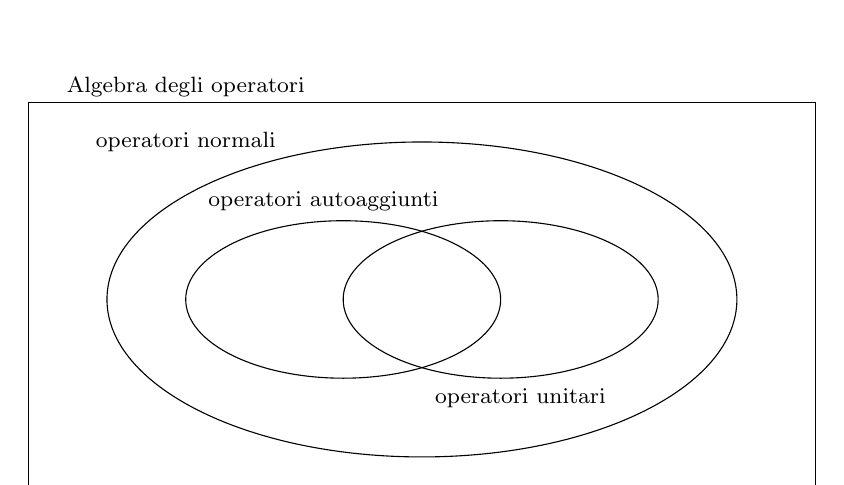
\begin{tikzpicture}
			\draw[] (-1, -1) rectangle ++(10, 5);
			\draw (4, 1.5) ellipse (4cm and 2cm);
			\draw (3 ,1.5) ellipse (2cm and 1cm);
			\draw (5, 1.5) ellipse (2cm and 1cm);
			\node (A) at (1, 4.2) {\footnotesize Algebra degli operatori}; 
			\node (B) at (1, 3.5) {\footnotesize operatori normali};
			\node (C) at (2.75, 2.75) {\footnotesize operatori autoaggiunti};
			\node (B) at (5.25, 0.25) {\footnotesize operatori unitari}; 
		\end{tikzpicture}
	\end{figure}
	Osserviamo che vale la seguente proposizione
	\begin{lemma}
		Se $T: V \to V$ è un operatore normale allora $\lambda$ è un autovalore di $T \iff \bar{\lambda}$ è un autovalore di $T^{\dag}$. Inoltre
		$$
			V_\lambda(T) = V_{\bar{\lambda}}(T)
		$$
	\end{lemma}
	\begin{proof}
		E' sufficiente mostrare che $\forall v \in V, T(v) = \lambda v \iff T^{\dag}(v) = \bar{\lambda} T(v)$. Osserviamo che se mostriamo che $T(v) = \lambda v \implies T^{\dag} (v) = \bar{\lambda} v$ allora segue che se $T^{\dag}(v) = \lambda' v \implies (T^{\dag})^{\dag} (v) = T(v) = \bar{\lambda'}v \implies T^{\dag}(v) = \bar{\lambda}v$: è dunque sufficiente mostrare una sola delle due implicazioni, per esempio la $\Rightarrow$. Si osserva
		$$
		T^\dag (v) = \bar{\lambda} v \iff (T^\dag(v) - \bar{\lambda}{v}, T^{\dag}(v) - \bar{\lambda}(v)) = 0.
		$$
		Dunque è sufficiente mostrare che vale la seconda proposizione per dimostrare questo lemma: siccome $T$ è normale, $T$ e $T^{\dag}$ commutano e dunque preso $v \in V_\lambda(T)$
		$$
		T T^{\dag} (v) = T^{\dag} T(v) = \lambda T^{\dag} (v) \implies T^{\dag}(v) - \bar{\lambda}(v) \in V_{\lambda}(T),
		$$
		d'altra parte abbiamo che, preso $w \in V_\lambda(T)$, la seguente relazione
		$$
		(T^{\dag}(v), w) = (v, Tw) =  (v, \lambda w) = \lambda (v, w) = (\bar{\lambda}v, w) \implies (T^{\dag}(v) - \bar{\lambda}v, w) = 0
		$$
		e prendendo $w = T^{\dag}(v) - \bar{\lambda}v$ (che sappiamo appartenere a $V_\lambda(T)$ siccome abbiamo visto che $T$ e $T^{\dag}$ preservano i rispettivi autospazi) avremo che
		$$
		(T^{\dag}(v) - \bar{\lambda}v, T^{\dag}(v) - \bar{\lambda} v) = 0 \iff T^{\dag}(v) = \bar{\lambda}v
		$$
	\end{proof}
	Possiamo generalizzare la dimostrazione fatta per gli operatori autoaggiunti anche per gli operatori normali
	\begin{theorem}[teorema spettrale per gli operatori normali in dimensione finita]
		Sia $V$ un $\mathbb{C}-$spazio vettoriale a dimensione finita munito di prodotto scalare $(\cdot, \cdot)$, sia $\mathcal{B}$ una base ortonormale e sia $T: V \to V$ un operatore normale. Allora $\exists \mathcal{B}'$ base di autovettori ortonormali rispetto al prodotto scalare 
	\end{theorem}
	\begin{proof}
	Preso $v \in V$ autovettore di $T$ allora possiamo decomporre $V$ come
	$$
		V = \text{Span}(v) \circled{+} (\text{Span}(v))^\perp
	$$
	e osservare che $\text{Span}(v)$ è $T-$invariante $\iff$ $T^{\dag}-$invariante per il lemma precedente. Ne segue allora che anche $(\text{Span}(v))^{\perp}$ è $T-$invariante e $T^{\dag}-$invariante: infatti preso $z \in (\text{Span}(v))^\perp$ chiaramente $(v, z) = 0$ e
	$$
	(v, T(z)) = (T^{\dag}(v), w) = (\bar{\lambda}v, w) = \lambda(v, w) = 0 \implies T(z) \in (\text{Span}(v))^{\perp}
	$$
	e similmente si mostra che $T^{\dag}(w) \in (\text{Span}(v))^{\perp}$, dunque $(\text{Span}(v))$ è $T-$invariante e $T^{\dag}-$invariante. Chiaramente $(T_{|(\text{Span}(v))^\perp})^{\dag} = T^{\dag}_{|(\text{Span}(v))^\perp}$ (dove il primo aggiunto va inteso rispetto a $(\cdot, \cdot)_{(\text{Span}(v))^\perp}$), da cui segue che $T_{|(\text{Span}(v))^\perp}$ è un operatore normale su $(\text{Span}(v))^\perp$ e procedendo per induzione si ottiene la tesi.
	\end{proof}
	\chapter{Quinta lezione}
	Nelle scorse lezioni abbiamo introdotto varie strutture:
	\begin{align*}
	&(V, (\cdot, \cdot)) \text{ sp. vett. con prod. scalare } \implies (V, ||\cdot||) \text{ è anche uno sp. normato } \implies \\
	&\implies (V, d) \text{ è anche uno sp. metrico}
	\end{align*}
	Nell'astratto potremmo in realtà dire che tutti queste $3$ strutture sono accomunate dal fatto di essere degli \emph{spazi topologici}. Adesso noi ci concentreremo nel dare alcune nozioni di topologia in spazi normati siccome sono quelli con cui lavoreremo, tuttavia bisogna tenere in mente che queste definizioni possono esssere "svincolate" dal concetto di norma.
	\begin{definition}[punto di accumulazione]
		Sia $A \subset V$, dove $(V, ||\cdot||)$ è uno spazio normato, e sia $\underline{v} \in A$, diremo che $\underline{v}$ è un punto di accumulazione di $A$ se
		$$
		\forall \varepsilon > 0, \exists v \neq \underline{v} \in A: || v - \underline{v} || < \varepsilon.
		$$
	\end{definition}
	\begin{remark}
		Non è necessario che $\underline{v} \in A$ (per esempio basti pensare alla frontiera di un insieme aperto, come la frontiera di una palla aperta $\subset \mathbb{R}^n$ di raggio $r$ e centrata in $x_0$: abbiamo che i punti che si trovano esattamente a distanza $r$ non appartengono all'insieme, ma si può comunque trovare un punto vicino "a piacere" ad ogni punto di frontiera).
	\end{remark}
	\begin{definition}[limite di funzione a valori in $V$]
		Sia $A \subset V$, dove $(V, || \cdot ||)$ e $(W, ||\cdot||')$ due spazio normati, sia $\underline{v}$ un punto di accumulazione di $A$ e sia $f: A \subset V \to W$ allora diremo che
		$$
			\lim_{v \to \underline{v}} f(v) = w \in W \iff \forall \varepsilon > 0, \exists \delta > 0: || v - \underline{v} || < \delta, v \neq \underline{v} \implies || f(v) - w ||' < \delta 
		$$
	\end{definition}
	A questo punto possiamo anche dare la nozione di continuità
	\begin{definition}[funzione continua in un punto]
		Sia $A \subset V$, dove $(V, || \cdot ||)$ e $(W, ||\cdot||')$ due spazio normati, sia $\underline{v}$ un punto di accumulazione di $A$ e sia $f: A \subset V \to W$. Se $\underline{v} \in A$ e
		$$
			\lim_{v \to \underline{v}} f(v) = w = f(\underline{v})
		$$
		diremo che la funzione è continua in $\underline{v}$, mentre diremo che la funzione è continua in $A$ se è continua $\forall x \in A$.
	\end{definition}
	\begin{prop}[unicità del limite]
		Se $\exists \lim\limits_{v \to \underline{v}} f(v) = L$ allora $L$ è unico 
	\end{prop}
	\begin{proof}
		Supponiamo per assurdo che esistano $l_1 \neq l_2 \in W$ tali che
		\begin{align*}
			&\lim_{v \to \underline{v}} f(v) = l_1 & &\lim_{v \to \underline{v}} f(v) = l_2
		\end{align*}
		allora sappiamo che $|| l_1 - l_2|| < \alpha$. Dunque per definizione di limite, sappiamo che $\exists \delta_1, \delta_2 > 0: || v - \underline{v} || < \delta_1 \implies ||f(v) - l_1 || < \frac{\alpha}{2}$ e $||v - \underline{v} || < \delta_2 \implies ||f(v) - l_2|| < \frac{\alpha}{2}$, dunque preso $\delta = \min\{ \delta_1, \delta_2 \}$ avremo che  
		$$
		|| l_1 - l_2 || \underbrace{\leq}_{\text{dis. triang.}} || f(w) - l_1 || + || f(w) - l_2 || <  \frac{\alpha}{2} + \frac{\alpha}{2} = \alpha.
		$$
		dunque $|| l_1 - l_2 || < \alpha$, il che è un assurdo.
	\end{proof}
	\section{Successioni}
	Una successione $\{ v_i \}$ con $i=1, \ldots, +\infty$ si dice successione di elementi di $V$ se $v : \mathbb{N}^{\geq 0} \to V$.
	\begin{definition}[limite di una successione]
		Sia $\{ x_i \}$ una successioni a valori in $V$. Diremo che $\exists \lim_{i \to +\infty} x_i = v \in V$ se $\forall \varepsilon > 0 \exists N \in \mathbb{N}: ||v - v_i|| < \varepsilon \forall i > N$.
	\end{definition}
	Una tipologia di successioni molto importanti sono le successioni di Cauchy (che ora definiremo formalmente), le quali sono delle successioni che "vorrebbero" avere limite (affermazione che verrà compresa per appieno nel momento in cui verrà affrontato il concetto di completezza e di completamento di uno spazio)
	\begin{definition}[successioni di Cauchy]
		Sia $\{ v_i \}$ una successioni a valori in $V$, diremo che essa è di Cauchy se
		$$
		\forall \varepsilon > 0 \exists N \in \mathbb{N}: \forall i, j > N, ||v_i - v_j || < \varepsilon.
		$$
	\end{definition}
	\begin{prop}
		Se $\{ v_i \}$ è una successione convergente allora è di Cauchy
	\end{prop}
	\begin{proof}
		Siccome $\{ v_i \}$ è una successione convergente a $v \in V$, fissato $\varepsilon > 0$, abbiamo che $\exists N > 0: \forall i > N, ||v - v_i||<\frac{\varepsilon}{2}$, pertanto
		$$
		\forall i, j > N, || v_i - v_j || \underbrace{\leq}_{\text{dis. triang.}} ||v_i - v || + || v_j - v || < \frac{\varepsilon}{2} + \frac{\varepsilon}{2} = \varepsilon.
		$$
	\end{proof}
	\begin{definition}[completezza]
		Sia $(V, d)$ uno spazio metrico, diremo che esso è completo se ogni successione di Cauchy è convergente.
	\end{definition}
	\begin{definition}[spazio di Banach]
		Sia $(V, d)$ uno spazio normato, diremo che esso è uno spazio di Banach se $(V, d)$ con $d$ distanza indotta da $||\cdot||$ è uno spazio metrico completo.
	\end{definition}
	\begin{definition}[spazio di Hilbert]
		Sia $(V, (\cdot, \cdot))$ uno spazio vettoriale munito di prodotto scalare, diremo che esso è uno spazio di Hilbert se $(V, d)$ con $d$ distanza indotta da $(\cdot, \cdot)$ è uno spazio metrico completo.
	\end{definition}
	\begin{definition}[palla aperta]
		Sia $v \in V$ e $R > 0$, definiamo $B(v, R) \subset V$ palla aperta come l'insieme
		$$
		\{ w \in V: ||w-v|| < R \}
		$$
	\end{definition}
	\begin{definition}[palla chiusa]
		Sia $v \in V$ e $R > 0$, definiamo $\overline{B(v, R)}$ palla chiusa come l'insieme
		$$
		\{ w \in V: ||w-v|| \leq R \}
		$$
	\end{definition}
	\begin{remark}
		$B(v, R) \subset \overline{B(v, R)} = B(v, R) \cup S(v, R)$ dove $S(v, R) = \{ w \in V: ||w-v|| = R \}$.
	\end{remark}
	\begin{definition}[insieme aperto]
		$A \subset V$ si dice aperto se $\forall v \in A \exists \varepsilon > 0: B(v, \varepsilon) \subset A$.
	\end{definition}
	\begin{prop}
		Se $\{ A_i \}$ è una collezione di insieme aperti, allora
		\begin{enumerate}[label=\protect\circled{\arabic*}]
			\item $\bigcup\limits_{i=1}^{+\infty} A_i$ è aperto;
			\item $\bigcap\limits_{i=1}^N A_i$ è aperto (\textbf{con} $N < + \infty$).
		\end{enumerate}
	\end{prop}
	\begin{proof} \hspace{1cm} \\
		\circled{1}: chiaramente se $x \in \bigcup\limits_{i=1}^{+\infty} \implies \exists j \in \mathbb{N}: x \in A_j$. Dall'apertura di $A_j$ sappiamo che $\exists \varepsilon > 0: B(x, \varepsilon) \subset A_j \implies B(x, \varepsilon) \subset \bigcup\limits_{i=1}^{+\infty} A_i$. $\circled{2}$: chiaramente se $x \in \bigcup\limits_{i=1}^N$ allora $\forall i \in \{ 1, \ldots, N \}, x \in A_i$, ma allora
		dall'ipotesi di apertura avremo che $\forall i \in \{ 1, \ldots, N \}, \exists \varepsilon_i > 0: B(x, \varepsilon_i) \subset A_i$. Posto $r = \min\{ \varepsilon_1, \ldots, \varepsilon_N \} \implies \forall i \in \{1, \ldots, N \}, B(x, r) \subset B(x, \varepsilon_i) \subset A_i \implies B(x, r) \subset \bigcup\limits_{i=1}^N A_i$. \\
		In entrambi i casi, la tesi segue dall'arbitrarietà di $x$. 
	\end{proof}
	\begin{remark}
		L'intersezione infinita di insiemi non è detto che sia un aperto: basti pensare all'intersezione di $\bigcup\limits_{i=1}^{\infty} (-\frac{1}{i}, \frac{1}{i}) = \{ 0 \}$ e chiaramente $\{ 0 \}$ è un chiuso siccome complementare dell'aperto $(-\infty, 0) \cup (0, +\infty)$.
	\end{remark}
	\begin{definition}[insieme chiuso]
		Sia $C \subset V$, diremo che $C$ è chiuso se $C^c = A$ è aperto.
	\end{definition}
	\begin{prop}
		Un insieme chiuso contiene tutti i suoi punti di accumulazione
	\end{prop}
	\begin{proof}
	Supponiamo per assurdo che $v$ sia un punto di accumulazione di $C$ e $v \not\in C$, allora sappiamo che $\forall \varepsilon > 0: \exists w \neq v: w \in C \text{ e } ||w - v||< \varepsilon$. Ma se $v \not\in C \implies v \in C^c = A$ aperto, dunque $\exists R > 0: B(v, R) \subset A$, ma allora fissando $\varepsilon = R$ abbiamo che $\emptyset \neq B(v, R) \cap C \subset C \cap C^c = \emptyset$, assurdo.
	\end{proof}
	Un concetto su cui adesso vogliamo concentrarci è il concetto di equivalenza fra norme
	\begin{definition}[norme equivalenti]
		Sia $V$ un $\mathbb{C}-$spazio vettoriale tale che, prese $||\cdot||_1, ||\cdot||_2 : V \to \mathbb{C}$, $(V, ||\cdot||_1)$ e $(V, ||\cdot||_2)$ sia uno spazio normato. Allora diremo che $||\cdot||_1$ e $||\cdot||_2$ sono equivalenti se
		\begin{equation*}
		\exists k, K \in \mathbb{R}_+ : k ||\cdot||_1 \leq ||\cdot||_2 \leq K ||\cdot||_1 \tag{$\ast$}
		\end{equation*}
	\end{definition}
	\begin{remark}
		Sebbene questa definizione possa sembrare, a prima vista, privilegiare la norma $||\cdot||_1$, osserviamo che la relazione $(\ast)$ di fatto implica che
		\begin{align*}
			\begin{cases}
				||\cdot||_2 \leq K ||\cdot||_1 \\
				k ||\cdot||_1 \leq ||\cdot||_2
			\end{cases} \implies \frac{1}{K} ||\cdot||_2 \leq ||\cdot||_1 \leq \frac{1}{k} ||\cdot||_2
		\end{align*}
		e, quindi, concludere che questa unilateralità della definizione è solo apparente. 
	\end{remark}
	Si può mostrare che le norme nel caso finito-dimensionale sono tutte equivalenti, il che implica che inducono tutti la stessa topologia: infatti, la nozione di limite di un qualcosa che tende a $0$ definita
	con una norma $||\cdot||_1$ sarà tendente a $0$ pure per la norma $||\cdot||_2$ siccome sarà possibile maggiorare la norma (e la tesi segue dal teorema del confronto). \\
	E' bene tener presente che è possibile anche solo maggiorare la norma, ovvero, prese $||\cdot||_1$ e $||\cdot||_2$ norme, trovare quel $K \in \mathbb{R}_{+}$ tale che
	$$
		||\cdot||_1 \leq K ||\cdot||_2.
	$$
	Nel caso infinito-dimensionale sarà spesso possibile maggiorare la norma e questo ci permetterà di dimostrare che alcuni fatti mostrati con la norma $||\cdot||_2$ sono validi anche per la norma $||\cdot||_1$ ma non inducono propriamente la stessa topologia (poiché altrimenti sarebbero equivalenti). Naturalmente, il fatto
	che due norme siano equivalenti \textbf{non} implica che non vi siano differenze fra l'usare una o l'altra: basti osservare anche solo graficamente come cambia il concetto di palla unitaria usando, rispettivamente, la norma euclidea, la norma del $||\cdot||_1 = \sum_i |z_i|$ e la norma infinito $\max_i |z_i|$.
	\begin{figure}[H]
		\centering
		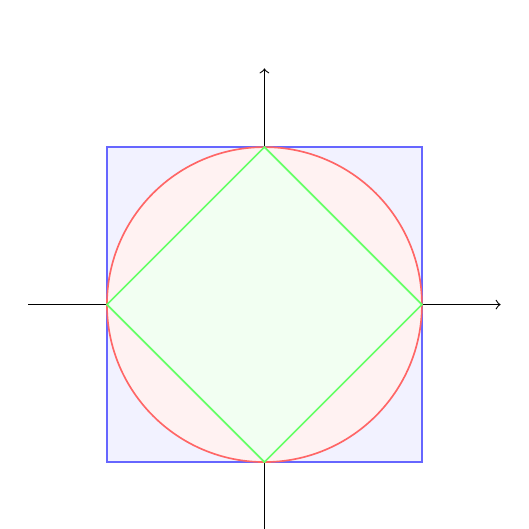
\begin{tikzpicture}
			% assi cartesiani
			\draw[->] (-3, 0) -- (3, 0);
			\draw[->] (0, -3) -- (0, 3);
			% palla euclidea
			\node (origin) at (0, 0) {};
			% palla della seconda distanza
			\filldraw[-,  color=blue!60, fill=blue!5, semithick] (-2, 2) -- (2, 2) -- (2, -2) -- (-2, -2) -- (-2, 2) -- cycle; 
			% palla della terza distanza
			\filldraw[color=red!60, fill=red!5, semithick] (0,0) circle (2);
			\filldraw[-, color=green!60, fill=green!5, semithick] (-2, 0) -- (0, 2) -- (2,0) -- (0, -2) -- (-2, 0) -- cycle;
		\end{tikzpicture}
		\caption{Palle unitarie con diverse distanze indotte da norme differenti. La regione rossa rappresenta la palla unitaria usando l'usuale distanza euclidea, la regione blu la palla dove si è utilizzata la distanza indotta dalla norma infinito mentre la regione verde la palla dove si è utilizzata la distanza indotta dalla norma del $\max$.}
	\end{figure}
	\chapter{Seconda esercitazione}
	Riprendiamo l'esercizio della scorsa volta. Abbiamo visto che la restrizione a $V_n$ dell'operatore $T$ permette di concludere che la sua matrice associata è
	\begin{equation*}
		\begin{bmatrix}
			1 & \frac{1}{\sqrt{2}} & \frac{1}{\sqrt{3}} & \ldots & \frac{1}{\sqrt{n}} \\
			0 & \frac{1}{\sqrt{2}} & \frac{1}{\sqrt{3}} & \ldots & \frac{1}{\sqrt{n}} \\
			\vdots & 0			   & \frac{1}{\sqrt{3}} & \vdots & \vdots \\
			0 & 0 & 0 & \ldots & \frac{1}{\sqrt{n}}
		\end{bmatrix}
	\end{equation*}
	La seconda richiesta dell'esercizio consiste nell'individuare come agisce l'aggiunto dell'operatore $T$ sul vettore $v$. Siccome $T$ è un operatore lineare, è sufficiente, naturalmente, vedere come questo agisce su una base dello spazio. Osserviamo che
	$$
		T^{\dag} e_p = \sum_{k=1}^{+\infty} (e_k, T^{\dag} e_p) e_k = \sum_{k=1}^{+\infty} (Te_k, e_p) e_k = \sum_{k=1}^{+\infty} \frac{1}{\sqrt{k}} e_k \chi_{\{k : k \geq p \}}(p) = \sum_{k=p}^{+\infty} \frac{1}{\sqrt{k}} e_k,
	$$
	dove si è introdotta la funzione caratteristica $\chi$ definita come
	$$
	\chi_S(x) = \begin{cases}
		1 & \text{se } x \in S \\
		0 & \text{se } x \not\in S.
	\end{cases}
	$$
	Osserviamo che negli spazi infinito-dimensionali non è detto che l'aggiunto sia ben definito per tutti i vettori, ovvero non è detto che l'aggiunto mi mandi dei vettori appartennti allo spazio di Hilbert $\mathcal{H}$ in vettori che appartengono sempre ad $\mathcal{H}$. \\
	A questo punto, possiamo individuare anche i possibili autovalori e autovettori osservando che
	$$
		T \Phi_k = \lambda_k \Phi_k \implies \Phi_k = \lambda^{-1}_k T \Phi_k.
	$$
	E' banale trovare lo spettro del nostro operatore: infatti, usufruendo delle proprietà del prodotto scalare, si osserva che
	\begin{align*}
		&x_k = \lambda^{-1}_k (\sum_{i=1}^{+\infty} (e_i, Tx_k) ) = \lambda^{-1}_k (\sum_{i=1}^{+\infty} (e_i, \frac{1}{\sqrt{k}} \sum_{j=1}^k x_j e_j)) = \lambda^{-1}_k ( \sum_{i=1}^{+\infty} \sum_{j=1}^{k} \frac{x_j}{\sqrt{k}} (e_i,e_j)) = \\
		&= \lambda^{-1}_k \sum_{i=1}^{+\infty} \sum_{j=1}^{k} \frac{x_j}{\sqrt{k}} \delta_{ij} = \sum_{i=1}^k \frac{x_i}{\sqrt{k}}
	\end{align*}
	ed è banale vedere che il vettore $(\underbrace{1, \ldots, 1}_{\text{k entrate}}, 0, \ldots)$ è autovettore relativo all'autovalore $\frac{1}{\sqrt{k}}$. 
	\section{Esercizio proposto}
	Posto $\Sigma(n) = \sum_{p=1}^n p = \frac{n(n+1)}{2}$ e preso l'operatore $T: \mathcal{H} \to \mathcal{H}$ tale che
	$$
		Te_n = \frac{1}{\sqrt{n}}
	$$
	%\addcontentsline{toc}{chapter}{Bibliografia}
	%\bibliographystyle{unsrt}
	%\bibliography{bibliography.bib}
	\chapter{Sesta lezione}
	Oggi ci concentremo sul concetto di insieme compatto e come possiamo usare tale definizione per mostrare che ogni funzione continua che mappa un compatto $C$ in $f(C) \subset \mathbb{R}$ assume massimo e minimo. Prima di procedere, è istruttivo soffermarsi su un esercizio
	che ci consente di intuire che lo spazio $C([a, b])$ che avevamo introdotto la scorsa volta non è completo con la norma $||\cdot||_1$. \\
	\begin{exercise}[lo spazio delle funzioni continue in un intervallo non è completo rispetto alla norma $||\cdot_1||$]
	\end{exercise}
		Consideriamo le funzioni $f: [-1, 1] \to \mathbb{C}$ continue e derivabili con derivata continua: ne deduciamo allora che essa siano limitate nell'intervallo $[-1, 1]$. Siano $||f||_1 = \max{|f(x)|}$ e $||f||_2 = \max{|f(x)|} + \max{|f'(x)|}$, allora abbiamo sicuramente che
		$$
		||f||_1 \leq ||f||_2 \, \forall f
		$$
		La norma $||f||_1$ viene quindi maggiorata da $||f||_2$ con $K = 1$, tuttavia non è possibile trovare un $k$ per cui $||f||_2 \leq K ||f||_1$. Inoltre, se prendiamo $g_n(x) = |x|^{1 + \frac{1}{n}}, g_n \in C^1([-1, 1]) \, \forall n \in \mathbb{N}$. Osserviamo che $g_n \to g(x) \to g(x) = |x|$ per $n \to +\infty$ nella norma $||\cdot||_1$. Infatti, limitandoci a $x > 0$, abbiamo che se poniamo $x = t^n, t \in [0, 1]$ allora $\max(t^{n}-t^{n+1})$ è in $t = \frac{n}{n+1}, 1-t = \frac{1}{n+1} \implies \max(t^n - t^{n+1}) \to 0.$ Ma $|x| \not\in C^1$ perché non derivabile per $x \neq 0$.
	\begin{definition}[insieme compatto]
		Sia $E$ un insieme, diremo che $E$ è compatto se per per ogni ricoprimento di insieme aperti esiste un sottoricoprimento di insieme aperti finito.
	\end{definition}
	\begin{prop}
		Se $E$ è un insieme compatto infinito, allora contiene almeno un punto di accumulazione.
	\end{prop}
	\begin{proof}
		Supponiamo per assurdo che $E$ non contenga alcun punto di accumulazione, allora sappiamo che $\forall v \in E, \exists r > 0: B(v, r) \subset E$ per cui solo $v \in B(v, r)$. Ma allora, posto $K = \{ B(v, r(v)) : v \in E \}$, allora possiamo
		estrarre un sottoricoprimento finito di $K$ che copre $E$, ma è chiaro che una collezione finita di palle aperte contenenti un solo elemento non sia in grado di coprire interamente $E$, siccome tale sottoricoprimento conterebbe solamente un numero finito di elementi.
	\end{proof}
	\begin{cor}
		Se $\{ x_k \} \subset E$ compatto, allora $\exists \{ x_{k_j} \} \to x \in E$.
	\end{cor}
	\begin{proof}
		Procediamo per assurdo. Sia $E$ un insieme compatto e sia $\{ x_k \} \subset E$ una successione: se non abbiamo una successione estratta convergente allora vuol dire che $\forall y \in E, \exists r_y > 0, n_y > 0 : \forall k > n_y, x_k \not\in B(y, r_y)$ (se non esiste nessuna estratta convergente allora la successione deve uscire da ogni palla). 
		Possiamo osservare che $X = \bigcup \{ B(y, r_y) : y \in E\}$ ma essendo $E$ compatto possiamo estrarre un sottoricoprimento finito: pertanto esistono $y_1, \ldots, y_m \in X : X = \bigcup\limits_{i=1}^m B(y_i, r_{y_i})$ ma allora, per quanto detto prima, sappiamo che $n$ sufficientemente grande (ovvero $n = \max{(n_{y_1}, \ldots, n_{y_m})}$) per cui $\forall i \in \{ 1, \ldots, m \}, x_k \not\in B(y_i, r_{y_i}) \implies x_k \not\in X$, il che è assurdo 
	\end{proof}
	Ora, siamo pronti ad enunciare il seguente risultato
	\begin{theorem}[teorema di Weierstrass]
		Sia $E$ un insieme compatto e sia $f: E \to \mathbb{R}$, allora $f$ assume massimo e minimo in $E$. Formalmente, diremo che $\exists x_{min}, x_{max} \in E : \forall x \in E, f(x) \geq f(x_\text{min})$ e $f(x) \leq f(x_\text{max})$. 
	\end{theorem}
	\begin{proof}
		Per caratterizzazione del $\text{sup}$ e del $\text{inf}$ sappiamo che esistono due successioni $\{ a_k \}$ e $\{ b_k \} \subset f(E)$ tali che $a_k \to \text{sup}(f(E))$ e $b_k \to \text{inf}(f(E))$. Senza perdita di generalità facciamo la dimostrazione per il massimo di $f$: siccome $\forall k \in \mathbb{N}, a_k \in f(E) \implies \exists x_k \in E : f(x_k) = a_k$. Ora, per la proposizione precedente, siccome $\{ x_k \} \subset E$ segue che esiste una sottosuccessione convergente $x_{k_j} \to x^* \in E$, ma allora
		$$
			f(x^*) = \lim_{j \to +\infty} f(x_{k_j}) = \lim_{k \to +\infty} f(x_k) = \text{sup}(f(E))
		$$
		dove la seconda uguaglianza discende dal fatto che $x_k$ è una successione convergente, dunque ogni sua estratta convergerà allo stesso $x^* \in E$. 
	\end{proof}

	\chapter{Settima lezione}
	
	In questa lezione vogliamo concentrarci sull'introdurre alcuni spazi a dimensione infinita che ricoprono una certa rilevanza.
\end{document}